%!TEX root = ../thesis.tex

\chapter{
  Illustrations of Human Movements
}
% Authoring Illustrations of Human Movements
% by Iterative Physical Demonstration

\newcommand{\systemname}{DemoDraw}
\newcommand{\phaseI}{Demonstration Interface}
\newcommand{\phaseII}{Refinement Interface}

Illustrations of human movements are used to communicate ideas and convey instructions in many domains, but creating them is time-consuming and requires skill.
We introduce a multimodal approach for people to generate these illustrations by physically demonstrating the movements.
Our \systemname{} system segments speech and 3D joint motion captured by a Kinect RGB-D sensor into a sequence of motion segments, each characterized by a key pose and salient joint trajectories.
Based on this sequence, a series of illustrations is automatically generated using a stylistically rendered 3D avatar annotated with arrows to convey movements.
During demonstration, users can also navigate existing illustrations using speech and amend or re-perform motions if needed. Once a suitable sequence of steps has been created, our system provides a \phaseII{} for finer control of visualization parameters.
In a three-part evaluation, we validate the effectiveness of the generated illustrations and the usability of both the \phaseI{} and the \phaseII{}.
Our results show that our participants could create 4-7 step-by-step illustrations from demonstrations in 22 minutes on average.

\begin{figure*}[t]
  \centering
  \includegraphics[width=\textwidth]{\demodraw/fig/teaser/teaser}
  \caption{\systemname{}: (a) multi-modal ``\phaseI{}'' to capture motion, verify results, and re-perform portions if needed; (b) conventional \phaseII{} for refinement and exploring other visualization styles; (c-d) examples of illustration styles.}
  \label{fig:demodraw_teaser}
\end{figure*}

%!TEX root = ../thesis.tex
\section{Introduction}

Popular online video-sharing websites such as YouTube have enabled the growth of a large community of users who share their knowledge and expertise in video tutorials. How-To videos demonstrate specific skills and procedures for tasks as varied as cooking, building a treehouse, or fixing a machine \cite{Torrey:2007he}.
These online tutorials help learners observe the manipulations and then put them into practice \cite{Torrey:2009fc}. However, in recording these videos, instructors often find it challenging to control the camera during demonstration.
%
Working with a cameraman who controls the device and viewpoints ensures that the video captures the movements that the audience would want to see, but it requires having a second person to direct the recording and work closely together with instructors. Many amateur users who mostly work alone, therefore, choose to self-record with one or more cameras. Camcorders can be set on a tripod to capture a static viewpoint, but it is hard to make sure whether users' actions are properly in frame at recording time. An alternative is to wear a head mounted camera to record what the instructors see. This may record unwanted and distractive head movements, making it difficult for the audience to watch. Additional camera views of the overall workspace might be needed to assist learners with understanding the context of demonstrated actions \cite{Fussell:2003te}.

\begin{figure}[t]
\centering
\vspace{0.15in}
\includegraphics[width=1.0\columnwidth]{\kinectograph/fig/teaser.pdf}
\caption{Kinectograph includes a Kinect camera to track user movement and a motorized dock to pan and tilt the camera so that the user (or their hand) remains centered in the recorded video. Here the device follows the user\'s hand while he is illustrating.}
\label{fig:figure1}
\end{figure}

Seeing these filming challenges, we would like to enable users to gain the flexibility of real-time camera control without requiring a dedicated camera-person. Our goal is to design a device that can automatically track and orient to film the tutorial instructors while providing lightweight manual controls. Existing video conferencing cameras and surveillance tools offer human tracking to provide full or partial automatic viewpoint control. Polycom\footnote{http://www.polycom.com/} designs video conferencing cameras that feature face recognition and voice detection to enable a group of users to talk in an office room setting. This approach assumes people's faces should be in the frame, which may not be true for instructional videos that focus on actions rather than ``talking heads.''
%
Automatic motion tracking is possible to always keep the user in view using visible markers \cite{Ranjan:2010} or wearable sensors such as infrared emitters by Swivl\footnote{http://www.swivl.com/}. However, instructors are unlikely to take such approaches to put on visible markers when demonstrating.
%
Researchers have been developing techniques to track specific targets using computer vision, including hands \cite{Ranjan:2008}, user movements \cite{Wilson:2012fb}, fast-moving objects (e.g., a Ping-Pong ball) \cite{Okumura:2011tr}, or regions in pre-defined spaces \cite{Ranjan:2007}. These usually require an expert defining heuristics of space regions or movement classifications ahead of time for the tracking program. On the contrary, we aim at proposing a new approach that does not have these issues, gives users flexibility in a home environment, and provides interactive control over the behavior of the camera tracking.
%
% TeleAdvisor assists a helper to remotely observe a physical task in real-time and provide instructions~\cite{Gurevich:2012ko}. However, the system is limited by the static camera view without automatic tracking.
%

We propose Kinectograph, a new device that enables semi-automatic camera control for users to self-direct camera orientation for demonstration tasks (Figure~\ref{fig:figure1}). Kinectograph serves as both the camera and the cameraman. It provides a motorized dock for a Kinect\footnote{http://www.xbox.com/en-US/kinect} sensor and a tablet-based user interface (separate from the camera) to switch between tracking regions at runtime based on their needs when demonstrating. Using skeleton tracking to follow the user’s movement, Kinectograph automatically pans and tilts the camera in real time. Users can define zoom regions that follow his actions to provide closeup views. Using a Kinect sensor, our system works in a common indoor setting and does not require the user to wear sensors or configure the environments. Kinectograph makes a novel contribution over the prior art in its mixed-initiative approach that offers various levels of automation and control to users at record time.

In this paper, we describe the user experience of recording with Kinectograph. We also describe design and implementation decisions. Finally, we review findings from a preliminary evaluation with 7 participants to study Kinectograph's usability of self-recording tutorials. All of the participants successfully created a demonstration video using our system without assistance and found it easy to interact with.

%\bjoern{I cut this out because you are missing the reference.}\new{In [insert citation here], they similarly use motors and a camera to automatically track and zooming in on users, but they do so in a conference setting. One of their system objectives is to unobtrusively track; however, our system focuses on providing enabling user's control in these tracking and zooming decisions for their DIY tutorials. In addition they only use facial and audio tracking and do not leverage the power of the kinect to do skeletal tracking.}

% Abhishek Ranjan, Jeremy Birnholtz, Rorik Henrikson, Ravin Balakrishnan, Dana Lee. (2010). Automatic camera control using unobtrusive vision and audio tracking. Proceedings of GI 2010 – the Graphics Interface Conference. p. 47-54.
%\pc{Where is the reference to the papers Bjoern sent? auto-tracking camera}

%!TEX root = ../thesis.tex

\chapter{Related Work}
\label{chapter_related_work}

While existing practices require tutorial authors to create instructions manually, HCI and Computer Graphics communities have introduced novel technologies for authoring tutorials, including automatic generation methods and interactive editing tools.
%
In this chapter, I survey state-of-the-art techniques for generating instructions for both software applications (Section \ref{related_software}) and physical tasks (Section \ref{related_physical}).
%
Furthermore, existing instructions are mainly offered in the forms of conventional media, such as static tutorials (print-outs or web) or videos. With software systems, \keyword{interactive tutorials} have been introduced for learners to interactively review instructional content. I will discuss various forms of such kind of instructions by prior research, which leads to a discussion on the remaining gaps in tool support for creating and navigating instructional content.
%
Finally, in Section \ref{related_videos}, I review the methods of video analysis and playback.

% -------------------------------------------

\section{Instructions for Software Applications}
\label{related_software}

\subsection{Input Event Visualization}

% real-time
Studies have shown that visualizing input events during user operations can provide better learnability of software applications~\cite{Dixon:2010fb}. Events can range from low-level, application agnostic input device events (e.g., mouse actions, cursor movements, or keyboard strokes) to higher level, application-dependent information (e.g., menu selections or UI component changes).
%
Commercial tools such as Mouseposé\footnote{\url{http://www.boinx.com/mousepose}} and ScreenFlow\footnote{\url{http://www.telestream.net/screenflow}} visualize mouse events and keystrokes with special effects, e.g., drawing a circle around a mouse cursor (see Figure~\ref{fig:related_realtime} top). These tools capture input information (e.g., mouse position and event type) and render visualization on top of the screen activities. This approach has been widely used by online video tutorial authors. However, it does not consider application context, which can be difficult for learners who want to follow specific instructions at a semantic level, such as observing a complete text field or drop-down menu option.
% Some further enable video editing techniques, including zooming in/out  and panning.

To visualization UI components (e.g., a checkbox, button, or editable text field), Dixon \ea{}'s Prefab~\cite{Dixon:2010fb,Dixon:2011:CHP:1978942.1979086} provides pixel-based enhancements in real-time by detecting target features, such as region corners. This semantic understanding of GUI elements enables component-based highlighting effects, such as afterglows~\cite{Baudisch:2006:PET:1166253.1166280} that visualize user operations (see Figure~\ref{fig:related_realtime} bottom left) and Bubble Cursor~\cite{Grossman:2005:BCE:1054972.1055012}, a target-aware pointing technique that suggests the nearest target (see Figure~\ref{fig:related_realtime} bottom right).

\begin{figure*}[t!]
  \centering
  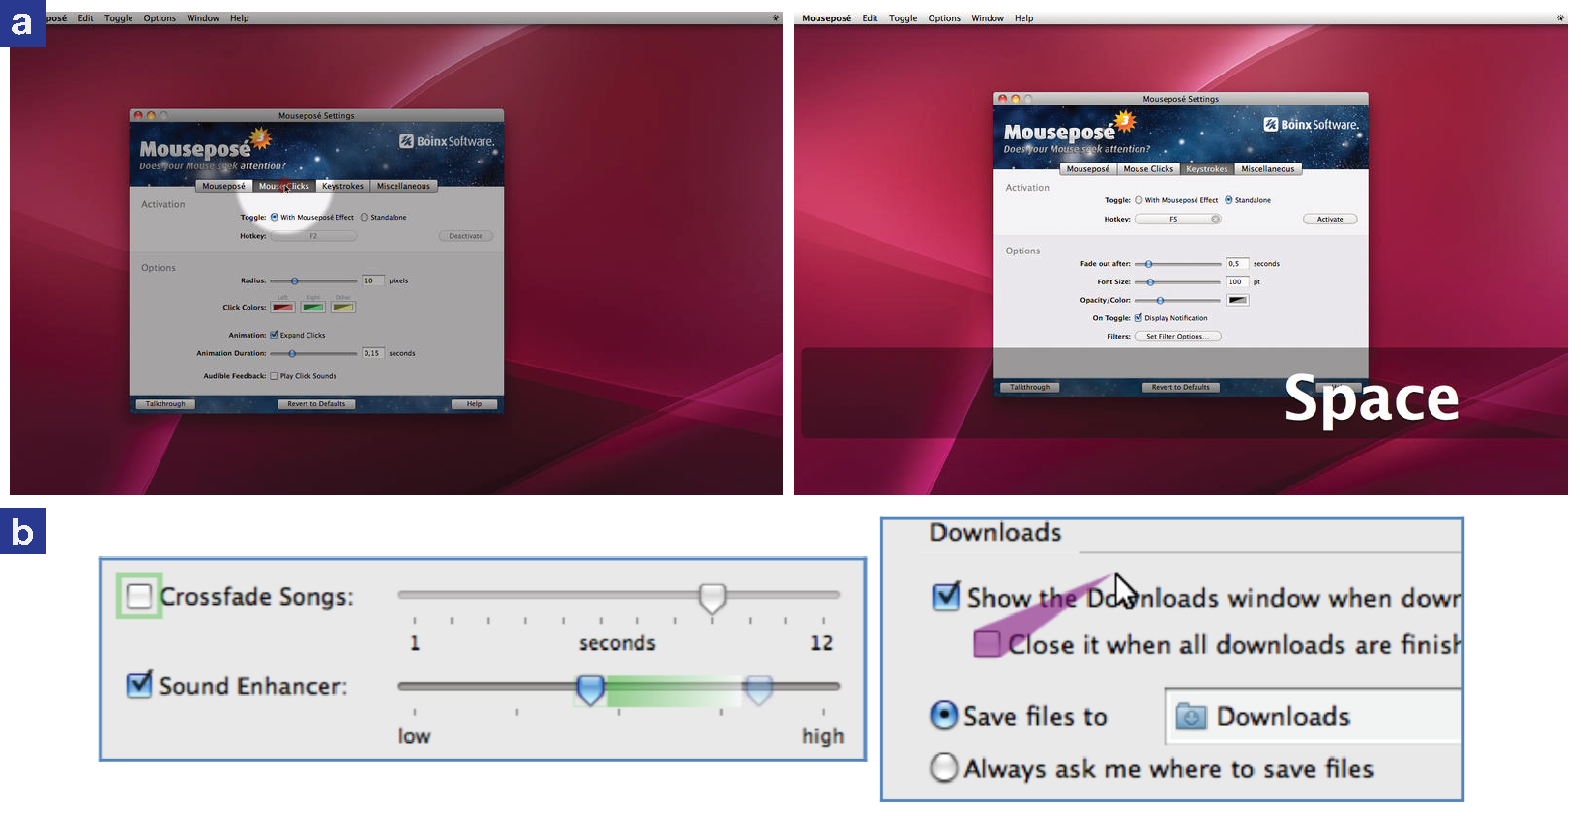
\includegraphics[width=0.7\textwidth]{\background/fig/realtime/realtime}
  \caption{Real-time visual enhancements on GUI applications: The top row shows how Mouseposé highlights a mouse cursor (left) and keyboard input (right); The bottom row presents Prefab~\cite{Dixon:2010fb}'s results of reverse engineering that identifies UI components and enables visualizations during author operations, such as afterglow~\cite{Baudisch:2006:PET:1166253.1166280} (left) and target-aware~\cite{Grossman:2005:BCE:1054972.1055012} (right) effects.}
  \label{fig:related_realtime}
\end{figure*}

\begin{figure*}[t!]
  \centering
  \includegraphics[width=0.6\textwidth]{\background/fig/software_viz/Nakamura_and_Igarashi}
  \includegraphics[width=\textwidth]{\background/fig/software_viz/Grabler}
  \caption{Example screenshots where mouse operations are automatically rendered, including (top) mouse move, drag, click, and wheel (a-d) by Nakamura and Igarashi~\cite{Nakamura:2008:ASV:1449715.1449721} and (bottom) application-specific operations (a-b), parameters (c-f), and manipulations (g-h) by Grabler \ea{}~\cite{Grabler:2009jj}.}
  \label{fig:related_events}
\end{figure*}

% in screenshots
The above methods enable real-time visualization of input events when operating an application, which are useful for following a video tutorial. However, they may not effectively present continuous actions, such as navigating a menu from the root to a sub-panel. For screenshot images in a static tutorial, visualizing input actions with motion arrows is a common technique to provide a sense of direction and start and end positions.
%
Researchers have investigated automatic approaches that capture and visualize these types of events in representative screenshots from author demonstrations. Nakamura and Igarashi~\cite{Nakamura:2008:ASV:1449715.1449721} proposed a capturing and rendering system independent to GUI applications. Their system logs mouse events of a software demo process, including mouse moving, dragging, and clicking. Operations are rendered as markers and arrows on screenshot images to present the linear event history (see Figure~\ref{fig:related_events} top).
%
Grabler \ea{}'s approach~\cite{Grabler:2009jj} further annotates a screenshot with bounding boxes and call-outs, which help learners identify parameters and options of software functionalities (see Figure~\ref{fig:related_events} bottom).

% summary
Our systems adopt some of these successful techniques to enhance visual instructions. By capturing event information at both input device and application levels, we visualize author operations based on different playback modes.
%
During \emph{video playback}, MixT shows mouse trails and actions, and DemoWiz overlays glyphs and arrows to guide viewers from the current input action to the next.
%
In a \emph{static}, step-by-step tutorial, MixT renders screenshot images with mouse visualizations, such as highlighting a drop-down menu.

% -------------------

\subsection{Workflow Capturing and Tutorials}
In addition to visualizing input events, it is important to present the entire workflow in a tutorial and provide concise instructions.
%
Grabler \ea{}'s system~\cite{Grabler:2009jj} generates a step-by-step tutorial from author demonstration (see Figure~\ref{fig:related_static}). Designed for instructing image manipulation tasks, it includes textual description from templates, such as \iquote{Select the \textbf{path tool} from the \textbf{toolbar} to \textbf{create and edit paths}.} The generated text and annotated images of operations are presented in a document to describe a workflow. Their work is available as a Photoshop plug-in\footnote{Adobe labs. Tutorial Builder. \url{http://labs.adobe.com/technologies/tutorialbuilder/}}.
% analyzes the application context, including facial features and outdoor scenes in manipulated images.
%
Such demonstration-based approaches have been applied to generate instructions for software that involves complicated manipulations or gestures, including 3D mesh construction~\cite{Denning:2011fy} and touch-based mobile applications~\cite{Wang:2014:EAC:2556288.2557407}.
%
Beyond logging input events during an author demonstration, researchers have shown that workflows and software content can be acquired using computer vision from analyzing desktop regions~\cite{Yeh:2009dh,Chang:2011vd} and existing screencast videos~\cite{Banovic:2012kd}.

\begin{figure*}[t!]
  \centering
  \includegraphics[width=0.8\textwidth]{\background/fig/related_static/grabler}
  \caption{Example static tutorial automatically generated by Grabler \ea{}'s system~\cite{Grabler:2009jj}.}
  \label{fig:related_static}
\end{figure*}

To compare effects of individual operations in a workflow, showing a list of ``before'' and ``after'' thumbnails, video clips, and event timeline can be effective \cite{Grossman:2010jz}, especially for image manipulation tasks (see Figure~\ref{fig:related_comparison} left).
%
When there are multiple workflows that create similar results, a union graph and side-by-side documents are useful for comparing operations~\cite{Kong:2012:DTR:2207676.2208549} (see Figure~\ref{fig:related_comparison} right).

\begin{figure*}[t!]
  \centering
  \includegraphics[width=0.4\textwidth]{\background/fig/software_viz/Grossman}
  \includegraphics[width=0.55\textwidth]{\background/fig/software_viz/Kong}
  \caption{Instructional systems that help learners compare effects and similar tutorials using (left) before and after images (a) and event timeline (b) by Grossman \ea{}~\cite{Grossman:2010jz} and (right) operation union graph by Kong \ea{}~\cite{Kong:2012:DTR:2207676.2208549}.}
  \label{fig:related_comparison}
\end{figure*}

% summary
These systems provided insights on 1) automatic generation methods of step-by-step tutorials and 2) workflow presentations serving for different purposes. Our MixT system is built based on the Photoshop plug-in (Tutorial Builder) to acquire a step-by-step document with text descriptions. We enhance the static tutorial format by embedding instructional video clips for each operation that can be interactively reviewed.

This paradigm opens a design space to create new tutorial formats that can be interactively reviewed. In recent years, researchers have shown that learners using responsive video tutorials~\cite{Nguyen:2015:MST:2702123.2702209} and learning-by-doing activities~\cite{Kwon:2016:CEO:2858036.2858101} performed better in following instructions than using static or video tutorials.

% -------------------

\subsection{In-Application Support}

The above methods introduce innovative ways for learners to review workflows and instructions. However, reviewing these materials is often separated from operating a software application. Learners might have to switch between the main application they are using and a separate set of instructions, which could introduce a gap of evaluation (\iquote{Am I doing this right as the instructions explain?}) and a gap of execution (\iquote{How do I perform the action that the instructions describe?}).
%
Researchers have proposed another approach to provide ``in-application'' assistance, often in real-time, in a specific application context.

There has been a considerable amount of research devoted to offering interactive help to support learners comprehend the functionalities while operating an application.
%
Crystal~\cite{Myers:2006:AWW:1124772.1124832} enables software users ask questions about ``why'' something did or did not occur in an application.
%
Video snippets can be embedded in application tooltips to explain specific functionalities~\cite{Grossman:2010wr}, which were shown to be seven times more effective than conventional tooltips for completing unfamiliar tasks.

Interactive, step-by-step instructions can be integrated in several forms:
%
To help software users identify specific UI components, tutorials can be shown via a translucent colored ``stencil,'' which visually directs user's attention in an application~\cite{Kelleher:2005:STD:1054972.1055047}.
%
By tracking user's current operations, tutorials can be embedded in an application to provide instant feedback such as a check-mark or a percentage match~\cite{Fernquist:2011:SRE:2047196.2047245}, automatically replayed to present the corresponding video instructions~\cite{Pongnumkul:2011ju}, or be shown as ambient help~\cite{Matejka:2011:AH:1978942.1979349}.
%
Instructions can be captured from demonstration as ``scripts'' for step-by-step navigation~\cite{Bergman:2005:DocWizards}. In-application controls~\cite{Lieberman:2014:SML:2557500.2557543} and game elements~\cite{Li:2014:CGM:2556288.2556954, Dontcheva:2014:CCL:2556288.2557217} can further engage users in learning.

As tutorials are built for a broader community with a set of authors and learners, content can be dynamically updated within a community based on user contribution~\cite{Lafreniere:2013ff,Matejka:2009:CCR:1622176.1622214, Bunt:2014:TPI:2556288.2557118}.

Our work focuses on authoring tools to create novel tutorial format designs, not the learning support. We see opportunities of combining our approaches with in-application guidance. For example, a video clip from a MixT tutorial can be automatically replayed when a system detects a slowdown of a learner's progress on a specific step. However, we do not claim contribution in this direction.

% These projects show how effective instructional representations can assist learners in learning or executing tasks. Our goal is to further study new formats that incorporate advantages of several formats of multimedia, including images, text, and videos, and in turn enhancing the learning experience for a variety of tasks.

% * define ``automatic''
% Note: MixT tutorials are automatically rendered from manual demonstration, not automatically generated.

% To provide real-time assistance, it is important to recognize the user activities during a task performance. Several domains have been widely studied, including software operations, scene recognition, and object tracking in a physical world.

% -------------------------------------------

\section{Instructions for Physical Activities}
\label{related_physical}

The above approaches of tracking a software demonstration open the door to enable interactive tutorials that can respond to user progress. However, understanding user behavior in the physical world, rather than in software, remains challenging.
%
How do technologies track humans and objects in a space to support real-time feedback? What are the available authoring techniques to generate instructions for physical tasks?
%
This section discusses the challenges from four perspectives, including tracking activities, authoring instructions, presenting guidance, and enabling interactive instruction following in a real world.

% -------------------

\subsection{Tracking Physical Activities}
To record activities and provide responsive feedback, a computer system needs to detect user operations and objects in real-time.
%
Computer vision techniques can automatically track specific physical targets shown in a video for interactive applications. These include three major categories:

\begin{itemize}
  \item \textbf{Tracking objects}. Common techniques include:
  1) Track specific \emph{colors} or visual features of pre-defined objects. Examples include tracking a fast-moving Ping-Pong ball for automatic camera control~\cite{Okumura:2011tr} or paper puppets for creating animation~\cite{Barnes:2008:VideoPuppetry}.
  %
  2) Track both \emph{colors and depths} of objects, which could obtain a better understanding of the objects' positions in a 3D world. The information can be useful for activities involved object manipulations, such as block or toy assembly tasks~\cite{Gupta2012DuploTrack,Wu:2016:ARI:2856400.2856416} and 3D puppet control~\cite{held20123d}.
  %
  3) Track \emph{motion-capture markers}. The most common method is to attach reflective markers to an object's surface. This enables accurate, responsive capturing, such as to record an animator's continuous movements~\cite{Dontcheva:2003:LAC:1201775.882285}.
  %
  \item \textbf{Tracking humans}. Targets include \emph{faces} (e.g., to show a close-up of a speaker during video conferencing~\cite{Ranjan:2010}, provide real-time camera control guidance when filming an interview video~\cite{Carter:2010}, and capture facial performances~\cite{Shi:2014:AAH:2661229.2661290,thies2016face}), \emph{hands} (e.g., to enable gestural control~\cite{taylor-siggraph2016} and camera control of a repair task~\cite{Ranjan:2008}), and \emph{user movements} (e.g., to provide augmented information~\cite{Wilson:2012fb,Anderson:2013:YEM:2501988.2502045}).
  %
  Motion-capture markers are often used to accurately track actors in professional filmmaking. However, since markers are visible in a camera view, visual effects (VFX) are necessary to post-process a video recording.
  %
  \item \textbf{A combination of the above}, such as reconstructing a 3D scene of a player throwing a basketball~\cite{dou-siggraph2016}.
\end{itemize}

Some of these vision-based systems require a high-speed camera~\cite{Okumura:2011tr} or a RGB-D camera~\cite{Gupta2012DuploTrack,Wu:2016:ARI:2856400.2856416,held20123d,Wilson:2012fb,Anderson:2013:YEM:2501988.2502045,dou-siggraph2016}, while some require users to wear reflective markers~\cite{Ranjan:2008}.
%
Other non-vision tracking methods rely on sensors attached to an object or human, including GPS sensor~\cite{HexoDrone} and radio frequency wireless signals~\cite{Nguyen:2016:ICR:2935620.2935632}. These are often used for tracking a moving target in a larger space, such as a flying drone.
%
Finally, if video content is difficult to be extracted, crowdsourcing algorithms have been introduced to structure step-by-step videos by online workers~\cite{Kim:2014:CSI:2611222.2556986}.

% summary
The detection mechanisms from these systems inspired us to design interactive systems that can react to authors' activities without requiring users to carry  a sensor. For examples, Kinectograph and DemoDraw track authors' body parts using a Kinect sensor that has been widely available to consumers.
%
However, tracking technique for high-level information, such as the \emph{intent} of a certain action, is yet lacking. Therefore, when automatic activity recognition is difficult, we include authors in a loop to annotate a task. DemoCut provides an annotation interface for describing DIY videos; DemoDraw provides a multi-modal interface to label continuous body movements.

% These methods usually require an expert defining heuristics of space regions or movement classifications ahead of time for the tracking program.

% -------------------

\subsection{Authoring Instructions for Real-World Tasks}

We identified two major approaches to create instructions for physical tasks: model-based and demonstration-based generation.
%
A \emph{model-based} system analyzes the structure of an object or a task and renders instructions.
%
The approaches by Feiner and Seligmann~\cite{feiner:1985:AEA:1299975.1300548,Seligmann:1991:AGI:127719.122732} considered communicative intent and rules of object manipulation to create 3D illustrations. Their automatically-generated results showed that actions such as snapping latches can be effectively expressed by motion arrows and a cutaway view.
%
By analyzing object geometry and other attributes, Agrawala \ea{}'s~\cite{agrawala2003designing} system automatically renders step-by-step assembly instructions, e.g., for furniture and toys (See Figure~\ref{fig:related_models} left).
%
Technical diagrams can also be generated, such as an exploded view that explains mechanical assembly parts~\cite{li2008automated} and motion illustrations that describe how individual parts are operated~\cite{mitra2010illustrating}. Parts are highlighted using colors, often labeled with text; Casual chain sequence of mechanical interaction can be shown as a list of highlighted figures, annotated with motion arrows (See Figure~\ref{fig:related_models} right).
%
Reversely, an existing technical document can be automatically analyzed and transfered into 3D animation by parsing the parts, orientation, and visual annotations~\cite{Mohr:2015:RTD:2702123.2702490}.

\begin{figure*}[t!]
  \centering
  \includegraphics[width=0.3\textwidth]{\background/fig/model_generation/furniture}
  \includegraphics[width=0.5\textwidth]{\background/fig/model_generation/chain}
  \caption{Example instructions automatically generated by Agrawala \ea~\cite{agrawala2003designing} (left) and Mitra \ea~\cite{mitra2010illustrating} (right) using model-based approaches.}
  \label{fig:related_models}
\end{figure*}

A \emph{demonstration-based} system records an author's physical demonstration of a workflow. The captured materials can be either automatically analyzed by the system or manually edited by an author to create instructions.
%
One approach is to employ templates to help users capture sequences of distinct shots (e.g., Snapguide\footnote{\url{http://snapguide.com/}}) or provide a limited set of operations to record specific moments (e.g., adding or removing a part in a block-assembly task~\cite{Ranjan:2007,Gupta2012DuploTrack}).
%
Another approach is to provide an interface to support authors capturing multimedia materials during or after a demonstration, such as using a head-mounted capturing device~\cite{carter2015authoring}. For certain tasks, new recording devices need to be specially designed, such as an integrated device that includes an IR camera to capture a knitting process~\cite{Rosner:2008:SAK:1409635.1409682} and a turntable to record the building process of a DIY project~\cite{Tseng:2015:SPT:2771839.2771869}.

% summary
In this dissertation, we support a wide variety of how-to tasks from craft to home repair and cooking where automatically tracking user activities is not yet completely possible. Since these domains often involve author creativity and personal styles, we opt for the demonstration-based approach.
%
DemoCut, Kinectograph, and DemoWiz each allows authors to perform a physical demonstration in front of a camera, while semi-automatically capturing the activities.

% -------------------

\begin{figure*}[t!]
  \centering
  \includegraphics[width=0.4\textwidth]{\background/fig/ar/authoring}
  \includegraphics[width=0.41\textwidth]{\background/fig/ar/following}
  \caption{TeleAdvisor~\cite{Gurevich:2012ko} provides an authoring interface (left) for an instructor to guide a remote worker through a repair task (right).}
  \label{fig:related_teleadvisor}
\end{figure*}

\begin{figure*}[t!]
  \centering
  \includegraphics[width=0.55\textwidth]{\background/fig/ar/technical_document}
  \caption{Work by Mohr \ea{}~\cite{Mohr:2015:RTD:2702123.2702490} automatically analyzes a technical document and augments a machine with AR animation in 3D.}
  \label{fig:related_ar_annotation}
\end{figure*}

\subsection{Presenting Guidance}
To help learners perceive instructions for physical tasks, we discuss how guidance can be displayed in a 3D world. There are four main approaches to present real-time guidance.

First, rich information can be shown via an \emph{external display} placed next to the work area. Several applications adopt this method, including cooking~\cite{Uriu:2012:PRM:2207676.2207695} and block assembly tasks~\cite{Gupta2012DuploTrack,Wu:2016:ARI:2856400.2856416}. However, a learner may often switch his or her attention between the task and the instructions. To better blend the information into activities, Knibbe~\ea{} designed a display-embedded table as a physical workspace that monitors, records, and assists users~\cite{Knibbe:2015:SMI:2817721.2817741}. In this way, workers can review the information on the desktop while making a project.

Second, information can be \emph{overlaid on top of the work area} through a projector. Examples include supporting remote repair tasks~\cite{Gurevich:2012ko} (see Figure~\ref{fig:related_teleadvisor} right), assembly tasks~\cite{Kirk:2006:CRG:1124772.1124951}, cooking~\cite{Ju:2001:CIC:634067.634227}, and piano learning~\cite{Xiao:2016:IEI:2858036.2858577}.
%
For tasks such as dance movements, guidance can be shown on an augmented mirror that learners constantly focus on~\cite{Anderson:2013:YEM:2501988.2502045}.
%
This method can effectively present instructions at a location that can be viewed by a learner during a task. However, this often requires a specific indoor environment setup and a calibrated projector, which is not scalable.

Third, information can be \emph{augmented through a head-mounted display or a mobile phone} accessed and viewed by individuals. Researchers have shown AR applications that provide visual highlights for machine maintenance~\cite{Henderson:2011ff,Mohr:2015:RTD:2702123.2702490} (see Figure~\ref{fig:related_ar_annotation}), enable interactive touring in a city~\cite{Feiner1997}, explain product functionalities~\cite{MagicLens}, and present dynamic UI or information based on head orientation~\cite{Zhang:2014:HHO:2659766.2659773}.
%
Compared to the previous approach that projects information onto a public space, this method allows learners to access information individually. Multiple users can interact with an augmented system at the same time. However, learners have to wear or hold a device, which might limit their mobility while performing a task.

Last, for specific tasks, information can be conveyed \emph{directly via target objects}. Haptic feedback has shown to be useful to help learners capture guidance while focusing on the physical tasks, such as for sculpturing~\cite{Zoran:2013:FFD:2470654.2481361,Agrawal:2015:PPS:2807442.2807505}, building multi-material assemblies~\cite{Schoop:2016:DSS:2851581.2892429}, and learning Frisbee~\cite{Solomon:2014:UTI:2540930.2540965}. Visual cues such as LED patterns shown on a device can help direct user's attention~\cite{Solomon:2014:UTI:2540930.2540965,Vasey:2016:HHR:2897839.2927404}.
%
This approach is task-specific and can be difficult to generalize to other task domains.

\subsection{Providing Interactive Guidance}
% \subsubTitleBold{Responding to Learners' Progress}
Finally, we discuss how assistive technologies track a learning process and support interactive guidance. Providing responsive feedback requires an understanding of learners' activities. For specific tasks such as block assembly~\cite{Gupta2012DuploTrack,Wu:2016:ARI:2856400.2856416} and dancing~\cite{Anderson:2013:YEM:2501988.2502045}, learners' progress can be accurately tracked in 3D. This enables a tutorial system to provide real-time information about the current learner state, e.g., where to place the next block to the current model or suggested adjustment on a dance pose.
%
However, as we discuss earlier, tracking activities at the instruction level for real-world tasks is still lacking. Therefore, the majority of the systems provided user interfaces for learners to navigate instructions.
%
For a pair learning scenario, a remote instructor can manually provide instructional input based on the learner's progress that he or she sees, such as highlighting a component for remote repair tasks~\cite{Gurevich:2012ko,Kirk:2006:CRG:1124772.1124951} (see Figure~\ref{fig:related_teleadvisor} left).

Our work focuses on designing tools for tutorial authors to create instructions from demonstrating a task. DemoCut is designed for authoring instructions after the capture time. Kinectograph provides an control interface on a Tablet device for authors to carry and place in a space. DemoDraw's demonstration interface is similar to Anderson \ea{}'s~\cite{Anderson:2013:YEM:2501988.2502045} augmented mirror. But instead of overlaying instructions, we present a real-time rendering view of an author's movements via an external display placed in front of the user. We have not investigated tools for learners to follow a task.

% -------------------------------------------

\section{Working with Videos}
\label{related_videos}

Research in video understanding has introduced new ways to work with videos, including capturing, editing, and navigating. How do authoring tools help users record, organize, and edit necessary materials? What are the interaction techniques of reviewing one or multiple videos? In this section, we review these topics briefly.

% -------------------

\subsection{Capturing}
Tool supports at the capturing phase include:

\subsubTitleBold{Filming Suggestion}
Several research systems guide users at capture time to yield higher-quality videos. Real-time suggestions include framing of the subject or camera view (e.g., NudgeCam for interview videos~\cite{Carter:2010}) and actor's performance~\cite{Heer:2004ba,Davis:2003cu}. Shot suggestions can also be bootstrapped through user dialogs~\cite{Adams:2005}.
%
Patterns from expert storytellers and commonsense reasoning can recommend novice authors to capture materials and develop a story structure~\cite{Barry:2003:MCC:957013.957152,Kim:2015:MSN:2702123.2702507}.

\subsubTitleBold{Camera Control}
Viewpoints of stationary cameras can be automatically decided based on heuristics at record time to trace an actor, an area, or an object~\cite{Ranjan:2008,Okumura:2011tr}.
%
In recent years, quadrotor cameras enable a wide range of trajectories to capture a subject from different viewing angles. Roberts and Hanrahan~\cite{Roberts:2016:GDF:2897824.2925980} proposed an authoring tool for authors to plan and preview a camera trajectory. When being filmed, 3D gestures allow a person to control a quadrotor camera at the scene~\cite{Cauchard:2015:DME:2750858.2805823,Pfeil:2013:EGM:2449396.2449429}.

% summary
We proposed Kinectograph prior to these systems of quadrotor camera control. A recent commercial system has included a similar feature to track a moving user~\cite{HexoDrone}, which is based on GPS location instead of specific body parts.

% -------------------

\subsection{Editing}
Tool supports for video composition and editing include:

\subsubTitleBold{Annotation}
Researchers have investigated how to provide interactions that enable efficient, fluid annotation or labeling of video data. Examples include the EVA system~\cite{Mackay:1989} that encouraged authors to annotate materials at capture time. More recent interfaces leverage pen input (e.g., VideoTater~\cite{Diakopoulos:2006vt}) and touch or gestural input~\cite{Sarkar:2016:SCC:2858036.2858199}.

\subsubTitleBold{Story Composition}
When working with a repository of video clips, it can be challenging to compose a compelling story. Several new interaction techniques have been proposed:
%
A storyline can be created non-linearly based on relevant characters, emotions, and themes of the current edited clips~\cite{Shen:2009:WNE:1518701.1518825}.
%
Tangible controllers with a specialized table interface enable collaborative, non-linear editing~\cite{Bartindale:2012:STS:2207676.2207700,Bartindale:2016:TSS:2818048.2819929}.
%
Live authoring at capture time with a Tablet device allows an author to quickly organize clips and apply editing decisions~\cite{Freeman:2014:LLA:2611105.2557304}.

\subsubTitleBold{Computer-Powered Editing}
Frame-based editing of video is very time-intensive, as it forces users to operate at a very low level of detail. Editors can leverage \emph{metadata}, such as shot boundaries~\cite{Casares:2002dx} and transcripts~\cite{Berthouzoz:2012} that help users place cuts and transitions. This gives users higher-level editing operations at the shot level rather than the frame level.
%
Techniques of \emph{computer vision} and \emph{speech analysis} can automate certain visual effects, such as creating cinemagraphs~\cite{Bai:2012, Joshi:2012}, automatically-edited lecture videos~\cite{Heck:2007}, zoomable tapestries~\cite{Barnes:2010} and synopses~\cite{Pritch:2009vl}, or stabilizing shaky amateur videos~\cite{Liu:2011}.
%
Edits can take place during recording, such as switching to a close-up view of a person who is speaking~\cite{Ranjan:2010}.
%
When material can be reviewed in 3D such as character animation, camera angles can be optimized to render a new video by analyzing the actor data~\cite{assa2005action,assa2008motion}.
%
Finally, when video analysis is a matter of subjective taste, identifying salient frames or highlights can be outsourced to crowd workers~\cite{Bernstein:2011uj,Tang:2012:ECS:2207676.2208622}.

% summary
MixT, DemoCut, Kinectograph, and DemoDraw also use vision techniques for automatic editing. They differ from previous approaches in its focus on two particular application domains -- software and physical demonstration videos.
%
By focusing on a specific domain, MixT and DemoCut can make assumptions about the structure of the input and output video, such as the fact that there is a linear set of steps, and offer an interface and algorithms that make it easier to create high quality how-to videos.
%
Kinectograph makes editing decisions (e.g., pan-and-tilt, zooming) based on actor's body location for instructional videos.
%
DemoDraw includes a multi-modal interface where authors can annotate a motion recording using speech while physically performing movements.

% visual enhancement~\cite{Santosa:2013:DST:2470654.2466148}

% -------------------

\subsection{Navigating}
% Tool supports for video navigation include:
Automatic video control can follow user actions or preferences, such as segment playback when operating software applications~\cite{Pongnumkul:2011ju} or playback speed control~\cite{Cheng:2009:SUV:1518701.1518823}.
%
Videos can be navigated at the content level beyond a linear timeline, such as visualizing subject movements in a storyboard design~\cite{goldman2006schematic} or a continuous image mosaic~\cite{Teodosio:2005:SS:1047936.1047940} and enabling direct manipulation of a target in 2D~\cite{Dragicevic:2008:VBD:1357054.1357096,Goldman:2008:VOA:1449715.1449719,Karrer:2008:DDM:1357054.1357097} or 3D~\cite{Nguyen:2013:DMV:2470654.2466150}.
%
These techniques help viewers understand content flow and playback videos, and have been applied to screencast videos~\cite{Denoue:2013:RDM:2451176.2451190,Nguyen:2015:MST:2702123.2702209}.
%
To further navigate a long video or a set of videos, a canvas showing video tiles and timeline was shown to be 36\% faster than a conventional list view~\cite{Al-Hajri:2014:VPH:2611105.2557106}. A video digest is effective in browsing and skimming video content~\cite{Pavel:2014:VDB:2642918.2647400}.
% Lecture videos~\cite{Tang:2006:DIU:1111449.1111523},

These novel forms of video navigation inspired us to explore new visual and playback designs for revealing the video content.
%
MixT supports per-step video navigation embedded in a static tutorial.
%
DemoWiz augments a screencast video with novel visualization for following the content.
%
DemoDraw renders a series of human movements as concise motion illustrations.

% In contrast to these systems, we do not require the author to manipulate the camera or system during capture. Many leisure activities, such as home repair or cooking, require use of both hands or involve getting one's hands dirty, so camera manipulation is not possible. We use vision techniques for automatic recording and editing. It differs from previous approaches in its focus on particular application domains -- software and physical demonstrations. By focusing on specific domains, we can make assumptions about the structure of the input and output video, such as the fact that there is a linear set of steps or movements, and offer user interfaces and algorithms that make it easier to create high quality instructions.

%!TEX root = ../thesis.tex

\section{Principles and Methods}
% Motion Illustration
% \bjoern{this section is too long for the work it does - more than page! Shorten.}
% \dan{I did some trimming, now a few lines more than a column without comments (not counting figure).}
% \dan{The main takeways after reading this section should be: 1) the style of illustration our system supports matches what people actually need; 2) current practices are slow and/or require specialized skills; 3) automating the first part of the process is most important: generating (and experimenting with) keyframe illustrations with motion annotations from real time demonstrations. } \bjoern{Yes!}

To understand motion illustration design and production, we surveyed related literature, studied found examples, and interviewed individuals who create such illustrations.

\subsection{Design Principles}
%to evaluate five general methods
Cutting~\cite{cutting_representing_2002} argues that superimposing vector-like lines on an image satisfies four important criteria: it evokes a feeling of motion, the object undergoing motion is clearly represented, the direction of motion is clear, and the magnitude of motion is conveyed with reasonable precision. To complement this metaphoric representation, Cutting also argues for the more literal method of multiple stroboscopic images, which satisfies all criteria except clear motion direction. McCloud~\cite{mccloud_understanding_1994} provides further arguments and examples for using these methods in the field of comic illustration, and notes communication benefits when they are combined.

To examine how professional illustrators use motion lines and stroboscopic images, we gathered examples from sources like user manuals, gesture-based games, safety guides, % (e.g., for airplane safety or weight training),
illustration compendia (e.g.,~\cite{mijksenaar1999open}) and how-to books (e.g.,~\cite{greenberg2012sketching}).
%
We found Cutting's notion of vector-like lines are almost always rendered with an arrowhead % with of a clear head at the end of a line tracing the motion path.
in a variety of styles (heads, weights, colors) with strokes typically two-dimensional, smooth, and offset to avoid occluding the object.
Stroboscopic images can be overlapping or spatially distributed, and change in transparency or shading to convey time.
The most common style for depicting the object undergoing motion is a simplified black-and-white contour drawing, but filled silhouettes and flat-shaded colour can also be found -- using full color photographic detail is rare.
%
By carefully removing extraneous details, such techniques help readers focus on only the salient, abstract information.
% \bjoern{Add WHY - omit extraneous details to focus on salient features.}

% These methods can be used with the object undergoing motion rendered as a full color photo or as a stylized illustration with reduced detail. \dan{One or two sentence giving benefits of using illustrations over photos that adds more detail to the general argument in the introduction [references in Pat Hanrahan's lecture slides, maybe Buxton's sketching book ] } Early in the 90s, Dooley and Cohen designed a method to generate line illustrations from geometric model \cite{Dooley:1990:AIG:91394.91422, Dooley:1990:AIG:91385.91422}. This...

% http://vis.berkeley.edu/courses/cs294-10-fa13/wiki/index.php/Conveying_Shape:_Lines#readings

% NOTES

% - -

% Cutting (2002)
% (this article is amazing)

% 4 criteria for
% evocativeness: a feeling of movement
% clarity: can the object undergoing motion be easily identified
% direction: where is the object moving?
% precision: what is the magnitude of the motion?

% 5 general techniques to convey motion:
% dynamic balance: choose a pose to convey sense of movement (questionable direction, poor precision)
% affine shear: leaning into the direction of movement (evocative and somewhat clear, Cutting says direction is good(?))
%  motion blur (only evocative)
% stroboscopic images: “Motion as time discretely sampled” (poor direction (?) )
% arrows (action lines, speed lines), a more literal representation of the motion vector … Cutting says this is best: (evocative, clear, direction, precise)

% literal representations of motion (strobing, motion blur) and metaphorical (arrows, action lines)

% - -

% McCloud (1993)
% (need to read more)

% talks about benefits of combining stroboscopic and action-line (headless arrows)

% - -

% OpenHere

% Interesting history of the arrow (p19) -- it's a somewhat recent convention.

% kind of off-the-cuff description of different arrow and lines types on p102 (e.g. dotted lines indicate stages of movement)

% many techniques for visual instructions come form cartoons (e.g. lines for movement)

% - -

% Pat Hanrahan’s lecture slides (provides references to justify using illustration over photos ssaying  ``Illustrations often better than photographs, they enhance important features and emphasize unimportant detail''

% - -

% Buxton, Sketching Interaction

% (didn’t find anything relevant beyond comments about arrows being good for conveying motion … our work isn't really about sketching, we're illustrating.)


\subsection{Interviews: Methods Used In the HCI Community}
% https://docs.google.com/document/d/1TisNlsFUYQ3a-BuqryRv8qmyp3La-qLj-j3hN4PyVS8/edit
% \bjoern{The challenge here is that HCI researchers with Illustrator chops are MUCH closer to experienced designers than the general population. So using HCI authors to make an argument about ``non-designers'' is problematic. I took it out.}
% The examples we gathered above are produced by professional illustrators, but many other people create motion illustrations as part of their work --
% A central goal of our system is to empower individuals to rapidly create professional-quality motion illustrations.
To understand current creation methods, we conducted video interviews with six Human-Computer Interaction researchers with experience creating motion illustrations.
%
Conveying movement for interaction is common in HCI publications. We found 100 motion illustrations in 58 recent papers.

%We conducted interviews with 6 researchers with experience creating motion illustrations.
% We surveyed papers published between years 2005 to 2014 that contained motion illustrations in venues such as CHI, UIST, and MobileHCI -- we found whole-body motions, such as play in an interactive room and large display interactions; and  hand motions, such as smartphone interactions. We conducted video interviews with six authors of such papers about their process.

% and found
%100 motion illustration figures in 58 papers. From a pool of authors who created illustrations in two or more of these papers, we invited 6 to share their experiences (aged 25-43, all males: 3 professors, 2 industry researchers, 1 graduate student).
%Two participants had some design or art background.
%
%Interviews were conducted by video conference for one hour. The discussion focused on the creation process for 2 to 4 figures which we selected from the interviewee's papers. Selected figures for two interviewees were whole-body motions, such as game play in a room space and large display interaction; figures for the rest were hand motions, such as smartphone or hand-held device interaction.

\subsubTitleBold{Findings}
% in 3 categories: tools and creation process, motivations, and struggles
% Several authors emphasized the importance of concision and focus: they introduced important concepts via illustrations with unnecessary details excluded, like faces, clothing, and backgrounds. Establishing a consistent visual style was important to reuse graphic elements. %, especially for operating mobile devices.
%
All interviewees used a similar methodology to create motion illustrations: they took still photographs of people performing actions, traced outlines using Adobe Photoshop (4/6) or Illustrator (2/6), then added graphic annotations to convey motion. %One interviewee with design expertise sometimes drew illustrations from scratch.
%All interviewees mentioned the importance of iterating illustrations. Often preliminary versions were created for an early draft and refined later.
% 4 of the 6 interviewees used Photoshop, while 2 used Illustrator; 3 solely used a mouse while 3 used a stylus as a main input device.
%
All mentioned that it was time-consuming to set up scenes and poses, take and trace photos, then add details like arrow placement while maintaining a consistent style. Typical creation times were estimated between 10 minutes to a few hours.
They also noted how difficult it was to make adjustments: changing the pose or viewpoint essentially meant starting over again with new source photos and re-tracing.
Yet, identifying the best pose and viewpoint ahead of time is difficult and it often took several iterations to yield an illustration suitable for publication.
% \dan{I added the last sentence, Peggy please confirm that aligns with what you heard in the interviews ... I know at least I said that ;)}

\begin{figure}[t]
  \centering
  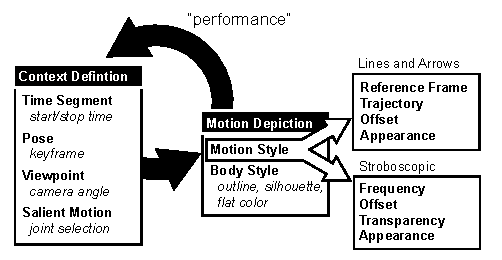
\includegraphics[width=\columnwidth]{\demodraw/fig/designdimensions}
  \caption{Canonical authoring workflow consisting of a Context Definition task then a Motion Depiction task. Design decisions associated with a task shown in bold with design parameters in italics.}
  \label{fig:designspace}
\end{figure}

\subsection{Design Space Goals and Workflow}

Based on the above, we derive a canonical workflow to motivate the central design goal for our system.
Authors face two primary illustration tasks (Figure~\ref{fig:designspace}):
\textit{defining the context} for portraying motion like the view of the body and salient aspects of motion;
and \textit{exploring a style of motion depiction} by choosing styles like lines-and-arrows or stroboscopic, then adjusting related style parameters.
These tasks and the underlying design parameters are highly interdependent, so authoring motion illustrations is necessarily an iterative process.
This means that changes to one task parameter often leads to re-evaluating and changing the other.
The problem with current methods, is that context is mostly ``performed'' using a time-consuming process of taking photos and manually tracing them.
%
Therefore, the central design goal of our system is to make context definition  low effort and iterative by using interactive demonstrations for automated context definition.

% enable low-effort iteration within, and between, the three identified tasks.

% %When creating illustrations, there are two primary tasks: 1) \textit{selecting the body context} and 2) body and motion \textit{depiction} (Figure~\ref{fig:designspace}).
% %\dan{I think ``context'' and ``depiction'' capture what people do, but maybe there are better terms.} \bjoern{yeah i don't understand them.}
% Performance capture involves recording suitable primary material to analyze and visualize. Identifying salient aspects
% %Selecting the body context
% involves segmenting a motion into steps, selecting key poses,
% %adjusting the camera angle to optimize the depiction of the pose and motion annotations,
% and identifying joints as salient motion for annotation. Depiction involves selecting a body visualization style, picking a motion visualization style (lines-and-arrows or stroboscopic), and adjusting many specific motion style parameters.
% These design parameters are all highly interdependent.
% %which is why the sequential and manual creation processes used by our interviewees is so time-consuming.


%Since current methods for the context setting task are time-consuming and inflexible, our system places extra focus on enabling rapid iteration.

Designing a system to capture interactive demonstrations of \textit{any} body movement also poses an input challenge.
Since  body movements form the demonstration itself, also issuing application commands with a body gesture introduces ambiguity.
Using a hand held device, touch screen, or any conventional input is not ideal since performing requires open space and full freedom of movement.
For these reasons, we use a multi-modal voice and gesture interaction style traced back to Bolt's Put-That-There~\cite{Bolt:1980:PutThatThere}. Like Bolt, we use voice for commands like \iquote{start} and \iquote{stop} with body movements providing command parameters in the form of the recorded demonstration, and for setting parameter context with utterances like \iquote{one, two, three, four} to label step-by-step segments.

%\peggy{We did not mention the reason we chose speech/voice for input. I briefly mentioned it in Pipeline in one sentence, but do we want to add a subsection here or mention in Introduction?}
%\dan{I added the paragraph above.}

% In addition, using manual techniques like photography or general purpose drawing tools like Adobe Illustrator means task parameters are highly under-constrained. This means the burden of upholding good design is placed on the non-expert user.
% A second goal of our system is to constrain the parameter space so that visualization principles are maintained.
% \dan{not sure if we do this second goal well}


% Lines: We may want to mention smoothing here? Several participants thought our system nicely smoothed the curves/arc (but should also straighten lines) even if their demo or Kinect mocap was not perfect.
% - Arrows: Double-headed arrows indicate repetition. DemoDraw does not adjust this automatically, but authors can manually change it to assign the intention.
% - Stroboscopic: also transparency? (had some meaning beyond appearance)
% - Sequencing: 1) DemoDraw generates the step-by-step diagrams based on motion segments, but also 2) Stroboscopic effect indicates the sequence of 2+ poses.

% \bjoern{Somewhere in the prior section or following section: Describe the design space of decisions one has to make to design an effective illustration. And argue that this is necessarily an iterative process where changes to one dimension may lead the designer to re-evaluate and change other dimensions. This is not possible with the current manual workflow starting with photos - authors are locked into a linear pipeline.}

% provide parameters, flexibility, direct manipulation, iterative design process



%!TEX root = thesis.tex
% User scenario using the DemoDraw system

\begin{figure*}[!t]
  \centering
  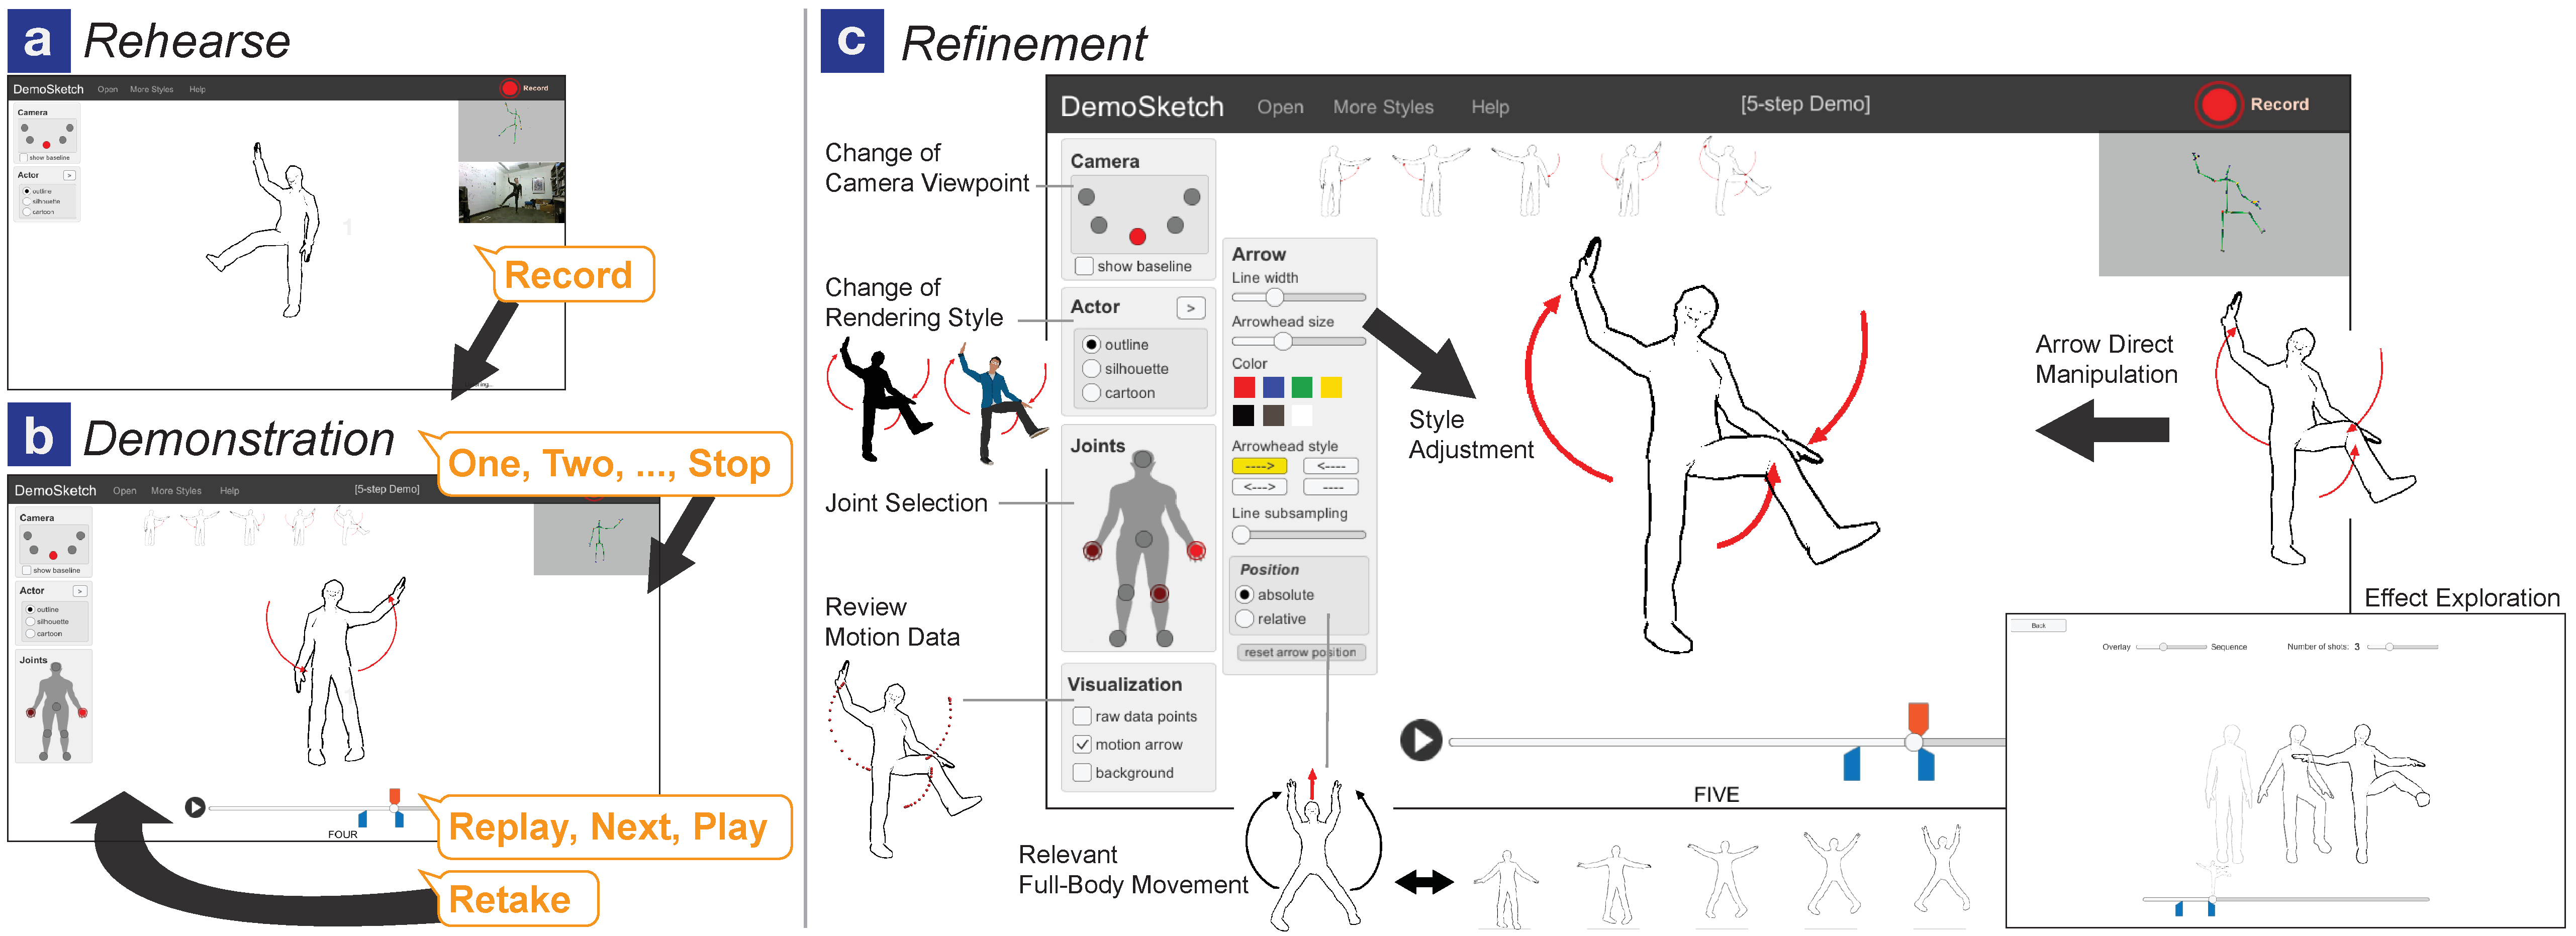
\includegraphics[width=\textwidth]{\demodraw/fig/ui/ui}
  \caption{\systemname{} authoring UI: Using the \phaseI{}, an author sees an avatar following her real-time movement (a). During recording (initiated by voice command ``Start''), real-time feedback shows the speech labels (b). Once a recording is completed by voice command ``Stop'', the motion visualization and a timeline are immediately available (c) for the author to review, and a step-by-step overview will be generated.}
  \dan{I changed figure start command to Start to match the video.}
  \label{fig:DemoDrawUI}
\end{figure*}

\section{Multi-Modal Authoring}
% \dan{Somewhere in this section need to justify need for motion re-taking and/or motion editing based on \textbf{three kinds of possible errors}: 1) user not happy with their own motion performance; 2) user not happy with quality of Kinect capture; 3) user not happy with system's motion segmentation or identified salience.}\bjoern{I'd add 4) based on illustration review, users decides to change performance to increase legibility.}

\systemname{} is designed for non-experts who cannot effectively or efficiently create concise motion illustrations motions using existing tools.
% This is achieved using two modes, the \phaseI{} and the \phaseII{}.
% \dan{The term ``phase'' implies a non-iterative sequential ordering. ``interface'' may not be good either if the UI is actually the same (I thought it was a bit different when they stood back for demonstration, but I guess not). Perhaps ``mode'' is best.)}
% \peggy{I agree and have changed the term in the paper}
To provide an overview of how the system works, we present a scenario in which a motion illustration author, Marie, creates instructions for an 8-step dance tutorial.

In her living room, Marie begins using \systemname{} with the \phaseI{} shown on her television by standing in front of a Kinect. In the center of the display, an avatar follows her movements in real-time (Figure~\ref{fig:DemoDrawUI}a).
 % with a smaller skeleton view and RGB video stream for recognition verification (Figure~\ref{fig:DemoDrawUI}-1b). \bjoern{I think you can get rid of the skeleton and perhaps also RGB video - those are debugging views for you.}
% \dan{just put one label for skeleton and RGB since these aren't a big focus}
This avatar is shown as an ``outline'' figure, but she could always change to different rendering effects like ``silhouette'' or ``cartoon,'' or select a different 3D human model later using our \phaseII{} (Figure~\ref{fig:DemoDrawRefinementUI}a).
% \dan{how does she select these while standing in front of the kinect? If she needs to use the \phaseII{} then let's talk about them there or have her pick them using the \phaseII{} before starting the demonstration.} \bjoern{yeah, i was wondering about this too}


\subsubTitleBold{Recording}
Marie starts recording her physical demonstration with the voice command \iquote{Start.} After a 3-second countdown, \systemname{} captures the position, orientation, and depth distance of her body (using Kinect's simplified 25 body joint model).
%
While demonstrating dance moves, Marie verbally indicates the count of each step with \iquote{one, two, three, and four,} just like she does when teaching a dance. The specific utterance is not constrained, Marie could use words like \iquote{right, left, shake, and clap.} A speech recognition engine captures these labels with timestamps and displays them in the interface (Figure~\ref{fig:DemoDrawUI}b).
Marie finishes recording by saying \iquote{Stop}.

\subsubTitleBold{Reviewing and Re-Recording}
After recording, \systemname{} automatically segments the motion around the speech labels and identifies salient joints. An illustration of the first step of Marie's demonstration is rendered with motion arrows, showing the path of the most salient joints. Figure~\ref{fig:DemoDrawUI}c presents an example illustration that shows how her right hand waves from bottom to the top, and the left on the opposite direction. She also notices three panels emerged: A timeline below shows the start, end, and key frame points used to generate the current illustration, a side panel shows the visualized joints; an step-by-step overview of step snapshots is created and added to a motion sequence list.
%
Marie can navigate to other illustrated steps by either saying \iquote{Next} or \iquote{Back}, or repeating one of the words she said during recording (like \iquote{three}) to skip to that corresponding step. To play an animation showing her continuous motion, she can say \iquote{Play} to play the current step only, or \iquote{Replay} to play the entire motion recording with each step visualization highlighted.

Once Marie reviews the steps, she realizes she should have exaggerated the hand motion in step 4. By saying \iquote{Retake Four,} Marie can re-record a partial sequence of movements including that step (e.g., redoing and saying ``Four'' and ``Five'').
When she ends the re-recording with \iquote{Stop}, the old illustration for that step is replaced with a new one (step four in this example) generated using the new motion recording.
%
% Furthermore, \systemname{} supports hand gestures for certain operations. For each step, \todo{Marie could adjust the start and end time of the motion using her left and right hands respectively.} By saying \iquote{Adjust}, she slowly moves her right hand to the right to extend the end time. She says \iquote{Done} to save the changes. She could always say \iquote{Cancel} to clear any recording or editing operation.
% No undo/redo
%
% TODO!! \dan{It would be so cool to have functionality to add and remove joints using the Kinect only: Marie finds that only her right hand was recognized as salient, but she wants a very subtle movement with her left hand to be shown too. She says \iquote{Add} while moving her left hand and the system adds her left hand's motion to the illustration. She can also say \iquote{Remove} to remove a joint from motion depiction.}

\begin{figure*}[t!]
  \centering
  \includegraphics[width=\textwidth]{\demodraw/fig/ui/refinement_ui}
  \caption{Using \systemname{}'s \phaseII{}, the author can refine the visuals (a) and explore more illustration effects (b, c).}
  \label{fig:DemoDrawRefinementUI}
\end{figure*}

\subsubTitleBold{Motion Depiction Adjustments}
Once Marie is satisfied with her demonstration, she walks out of the capture area to her desktop computer. The system automatically switches to the \phaseII{} by revealing post-processing panels in a standard graphical user interface (Figure~\ref{fig:DemoDrawRefinementUI}a).
% \dan{so there are two interfaces!}
Using this interface, Marie can adjust several design parameters:
% \dan{I rewrite these to match parameters in figure 2 and added some as well.}
the arrow appearance can be refined, including line width, arrowhead size, and color;
the arrow offset can be adjusted with direct manipulation dragging; %to avoid overlap with the avatar figure
the camera viewpoint can be adjusted by orbiting the camera to a side or three-quarter view;
the joints used for motion paths can be added or removed using a panel;
% \dan{I put viewpoint in the ``context task'' in prev section, so may need to say something about not all context parameters needs to be adjusted in \phaseII{}. }
and the smoothed motion trajectory can be toggled on and off.
%
She could also select a different key pose and adjust the start and end times of a motion segment by dragging the markers on the timeline.
% \dan{if no relative vs. absolute adjustments, we may want to remove ``reference frame'' from figure 2}
% \peggy{Add something about relative motion here.}
%
In addition, Marie could explore other illustration styles like stroboscopic rendering by selecting numbers of intermediate frames and how they render in one diagram (Figure~\ref{fig:DemoDrawRefinementUI}b).
%
These results can be exported to image files containing the final motion illustrations. %replace vector files - possible but not implemented

% \dan{are there other motion styles? I commented out text that suggested that but I didn't think there were more than these two.}
 % for one or more steps to illustrate the continuous movement in one figure. By choosing ``More Styles'' from the menu, a dialog reveals for her to explore the effects.

% Beyond rendering motion arrows, the user decides the visualize a list of poses to compare with. She selects the option``Sequence'' from the menu and generates a stop motion sequence, with a default of 3 frames (Figure~\ref{fig:DemoDrawUI}A). She adjusts the start and end points of the whole motion via the timeline markers, and changes the number of shots and their distance to overlay the figures together (Figure~\ref{fig:DemoDrawUI}B).

% \dan{I would leave these out because they aren't really about post-processing design parameters:
% She could also reveal the raw, smoothened motion paths to confirm the captured data (Figure~\ref{fig:DemoDrawUI}B).
% To make sure the motion arrow renders the actual motion, she toggles the option ``motion path'' to reveal the original trails;}

% \fixme{\subsubTitleBold{Output}
% Finally, Marie chooses to output the generated illustrations of 8 dance moves to one step-by-step diagram. \systemname{} also provides other output formats, including step-by-step animated clips with the 3D model (where the viewing angles can be adjusted), or video snippets from the Kinect camera view (which only provides the front viewpoint).}
% \dan{not sure we should even talk about output formats other than motion illustrations since they're the only focus of this paper. We can talk about other formats like video and even MixT in future work or discussion. If you agree, then this whole ``output section'' can be reduced to a final sentence of the previous paragraph.  }

%!TEX root = thesis.tex
% Pipeline of the DemoDraw system: technical details

\begin{figure}[t]
  \centering
  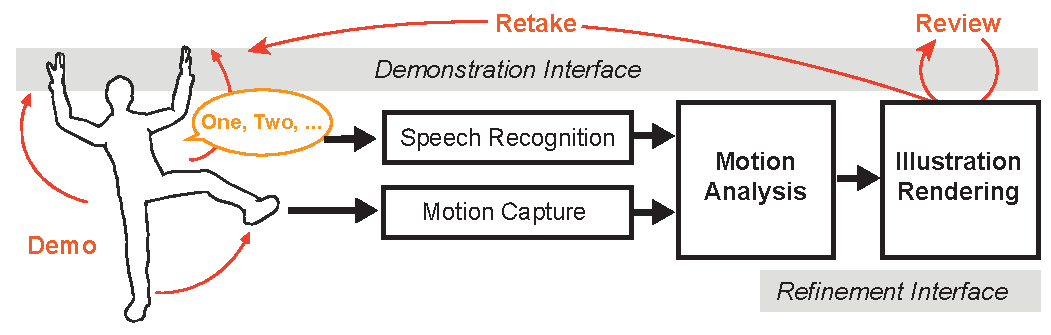
\includegraphics[width=0.8\columnwidth]{\demodraw/fig/pipeline/pipeline}
  \caption{\systemname{} System Components and Pipeline}
  % \dan{now that I understand the components better, we should emphasize motion capture component less since didn't make much contribution there.  I tweaked the figure to do this, and also highlighted the ``interaction pipeline'' (demo, review, retake) a bit better too.   }
  \label{fig:pipeline}
\end{figure}

\section{Generation Pipeline}

% \dan{I think we should downplay ``pipeline'' and emphasize ``system components'' ... pipeline sound very linear and non-iterative.}

%To support the described user scenario, we introduce our pipeline and system components shown in .
\systemname{} has four main components (Figure~\ref{fig:pipeline}):
%
a \emph{motion capture} engine to record joint data from the author's demonstration and apply it to a 3D avatar;
%
a \emph{speech recognition} engine to process speech input for commands and motion labels;
%
a \emph{motion analysis} algorithm to partition recorded motion and identify salient joint movements for each illustration segment;
%
and an \emph{illustration rendering} engine to visualize the avatar and motion segments with different effects.
% , and a module to handle user interaction.
%
% Our novel techniques enables motion segmentation by combining speech and motion inputs. Our interaction model allows users to modify the rendered illustrations interactively by demonstrations.
These components combine into an interactive and iterative system pipeline to translate demonstrations into motion diagrams.
A notable technical contribution is our motion segmentation algorithm combining speech labels and joint motion streams.
% \dan{I tweaked the two points above, old text is commented out in the tex}

% \dan{say something like our technical contribution is in motion segmentation (and maybe illustration rendering) }
%
\systemname{} is implemented using C\# in Unity 5. %\footnote{\url{https://unity3d.com}}.
It runs interactively on a Macbook Pro with Windows Bootcamp (2.5 GHz Intel Core i7 processor and 16 GB memory).
%
Below we describe the design and implementation of each component.

% ---------------------------------------------------------------

\subsection{Motion Capture}
% \dan{Call it ``Motion Capture'' component, with three sub components: Kinect, Avateering, and NPR}
% \bjoern{I moved NPR from capture to illustration rendering since it's a rendering technique.}
% \dan{good idea}

In support of our design goal to enable low-effort iteration within tasks, the motion capture component provides real-time feedback during demonstrations so authors can monitor their performance accordingly.
%\fixme{The raw joint data and RGB video stream are saved as csv and mp4 files for retrieval.}
%\dan{I put this here, but not sure we really need to state it at all. We don't really use the RBD video for anything either.}
% A central goal of our system is to enable average users to create illustration by physical demonstrations. As users might not necessarily have expertise to design illustration outcomes prior to a performance, it is important to provide real-time feedback for authors to observe the continuous motion captured effect and perform accordingly.
%
%\subsubTitleBold{Real-time Joint Data}
We capture position and joint angles of a simplified 25-joint skeleton using a Kinect2 sensor and the Kinect SDK 2.0. %\footnote{\url{https://dev.windows.com/en-us/kinect}}.
%Skeletal data of human body's 25 joints is captured in 3D, including head, shoulders, hands, and foot.
% At any given frame of motion capturing, our system gathers information about position, depth, and orientation values in meters for each of the 25 joints.
%Therefore, \systemname{} presents a 3D human model mirroring an author's movements in real-time while she stands in front of a Kinect sensor in a static, indoor scene (Figure~\ref{fig:pipeline}a).
%\dan{I commented a lot out here it didn't seem to add much beyond ``we capture using a Kinect'' (and just saying something like that is ok). }
%
%\subsubTitleBold{Motion Re-targeting}
The real-time joint data is applied to a generic 3D human model (an ``avatar'') using forward kinematics enabled by a modified Unity asset\footnote{\url{https://www.assetstore.unity3d.com/en/\#!/content/18708}}.
% \dan{I commented out a vague description of forward kinematics, I don't think we need it.}
% \bjoern{So the use of ``retargeting'' kinda raises a whole bunch of issues since motion retargeting is a big topic in animation. If bone lengths don't match between the actor's skeleton and the virtual model, contacts like clap or hand-on-head won't work. At a minimum state that we do not yet perform any smart retargeting to deal with changing segment lengths. I think the canonical reference is Gleicher~\cite{gleicher1998retargetting}.}
% \dan{yes, let's avoid saying ``retargeting''}

% When the motion data gets updated from the Kinect sensor, \systemname{} applies the joint information to a structured 3D human model (i.e., an ``avatar'') using forward kinematics in real-time. Given the human skeleton hierarchy from the body root (i.e., base spine) to the end of body parts (such as hand tips and feet), we compute the bone rotation angle to locate each joint to the target location in space. In this way, user can observe the avatar that follows her motion, which can also be viewed from any angle in a 3D space. This can be useful when user performs movements perpendicular to the Kinect camera \peggy{need a better way to frame this}.


% Based on our survey on existing practices of illustration design principles, it is important to make a character's appearance concise and clean. Often, outlining a human figure or showing in silhouette effectively preserves only essential information. Therefore, we apply Non-Photorealistic Rendering (NPR) techniques \cite{gooch1998non} to the 3D avatar in our engine that can be rendered and modified in real-time, including outline, silhouette, and flat-shaded colour (see Figure~\ref{fig:DemoDrawUI}-1d for examples).
% quaternion

% \subsubTitleBold{Implementation}
% This engine is implemented using Unity 5\footnote{\url{https://unity3d.com}} and the Kinect SDK 2.0 package\footnote{\url{https://dev.windows.com/en-us/kinect}} in C\#. Raw joint data and video stream from color frames are saved as csv and mp4 files for retrieval. Motion retargeting is achieved by a modification of a Unity asset\footnote{\url{https://www.assetstore.unity3d.com/en/\#!/content/18708}}. NPR shaders are applied to the 3D model for different rendering results.

% ---------------------------------------------------------------

\subsection{Speech Recognition}
Speech is used when recording a demonstration to label motions (e.g., ``one, two, ...'') and for recording and navigation commands (e.g. ``Start, Stop, Retake'' or ``Replay, Next, Play'') -- see Figure~\ref{fig:DemoDrawUI} for the speech commands that \systemname{} supports.
\dan{I made these consistent with new Figure 4}
%
We recognize both types of speech using the Microsoft speech recognition library\footnote{\url{https://msdn.microsoft.com/en-us/library/hh361572}} to process audio captured by the Kinect microphone array.
During recording, the start time, duration, and confidence of each motion label are logged for use in the motion analysis algorithm.
% https://msdn.microsoft.com/en-us/library/system.speech.recognition.recognizedaudio.starttime(v=vs.110).aspx
% \dan{how do you calculate delay? I thought this was a fixed constant determined by manual inspection.}
% \peggy{The api provides, but I didn't get to use it...}

%In addition, \fixme{a set of X voice commands} are recognized for non-sequential navigation .

%  addition to capturing and rendering user's continuous movements, \systemname{} considers instructor's existing practices of specifying motions using speech during a physical demonstration.
% By listening to the Kinect sensor's microphone array, \systemname{} integrates a speech recognition engine\footnote{\url{https://msdn.microsoft.com/en-us/library/hh361572}} to recognize user's speech input in real-time. Information of a detected spoken word, including the timestamp, delay, and confidence, is captured to be used for motion analysis and to support \systemname{}'s multi-modal interaction.
%
% Can implement: go more than one word and combine (e.g., turn to the right)

% ---------------------------------------------------------------

\begin{figure}[!t]
  \centering
  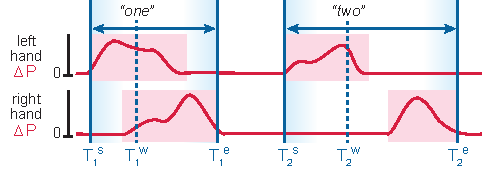
\includegraphics[width=0.8\columnwidth]{\demodraw/fig/motion_analysis/analysis2}
  \caption{Illustration of motion analysis algorithm (two joints shown due to space): significant moving periods of joint movements (pink) are mapped to speech labels to define motion segments (blue). Note the right hand period is mapped to \iquote{two} because it begins shortly after the left hand period.}
   \label{fig:segmentation}
\end{figure}

\subsection {Motion Analysis}
% \dan{Would be good to get a component name to include joint salience identification too.  ``Motion Segmentation and Joint Salience Identification'' component is too long, how about something more simple and general like ``Motion Analysis'' with subcomponents motion segmentation and joint salience.}

Our motion analysis algorithm translates a multi-part demonstration recording into a sequence of labeled time segments, each with one or more salient joint motions and a keyframe of joint positions for a representative body pose (see Figure~\ref{fig:segmentation} for an illustration of the approach).
Formally, given a set of $n$ speech labels $\{w_1, w_2, ..., w_n\}$ where each ends at latency-corrected time $\{T_1^w, T_2^w, ..., T_n^w\}$, our algorithm associates each speech label $w_i$ with a \emph{motion segment}, of which the start and end time are denoted as [$T_i^s$, $T_i^e$] where $T_i^s \leq T_i^w \leq T_i^e$. Each motion segment includes a set of $k$ salient joints $\{j_i^1, ..., j_i^k\}$ and keyframe time $T_i^{key}$ between [$T_i^s$, $T_i^e$].
It is then sent to the Illustration Rendering engine to create a motion illustration in a multi-part sequence.

Human motion segmentation and activity understanding has been well studied in computer vision and graphics \cite{Aggarwal:2011:HAA:1922649.1922653}. We adopted a spacetime approach to identify salient motion sequences in 3D space.
%
However, in our scenario such as dancing, movements may not necessarily encode a semantic meaning for automatic recognition, such as ``walking'' or ``throwing (a ball)'' in previous research. Therefore, our approach combines the user's speech labels, similar to a scene segmentation method used in DemoCut~\cite{Chi:2013:DGC:2501988.2502052}.
%
We make two assumptions about the synchronized data streams of speech labels and joint movements:
1) authors make short pauses between motions to be grouped, i.e., $T_i^e < T_{i+1}^s$, and
2) the speech label utterances overlap or closely occur with at least one joint motion;
% step-by-step movements are clearly segmented without an overlap.
%
These assumptions are practical since authors often pause for a moment to prepare for demonstrating the next movement in a step-by-step sequence.
% , or reposition their body without those movements being assigned to any label.

% where $T_s \leq T_w \leq T_e$,

% For a motion label detected by the speech recognition engine at time \(T_w\) (e.g., step ``One'' or a gesture ``Swipe''), \systemname{} automatically identifies an appropriate motion segment for visualization as follows: It analyzes the motion data in order to identify the start and end time of this segment [\(T_s\), \(T_e\)] where \(T_s \leq T_w \leq T_e\), a set of salient joints \({J_0, ..., J_n}\), and a representative pose at \(T_k\) associated with this speech label. Figure~\ref{fig:segmentation} shows one example of a right-hand movement segmented by the following approach: \bjoern{What instant in time does \(T_w\) represent? The beginning of a word? The end? Some time after the end of the word once recognition has completed? Seems fairly important - otherwise I have no idea if \(T_s \leq T_w \leq T_e\) is a reasonable assumption.}

% EUCLIDEAN DISTANCE
\subsubTitleBold{Motion Segmentation}
To determine a motion segment of [$T_i^s$, $T_i^e$] for each speech label $w_i$ that ends at $T_i^w$, we begin by identifying all \emph{moving periods} of significant joint movements (pink rectangles in Figure~\ref{fig:segmentation}) for 8 joints $J$: the 5 end-effectors (head, hands, feet), 2 knees, and the body root.
%
To filter jittery movements, joints are considered moving if smoothed inter-frame differences in absolute Euclidean distance are greater than a threshold.
%
Specifically, for each joint $j \in J$ of a frame $r$ at time $t$, the average difference in position between two adjacent frames $\Delta P = |P^r-P^{r-1}|$ is computed over the subsequent half second (15 frames).
%
If this moving average is greater than 0.05$m/s$, then joint $j$ of a frame is labeled as ``moving'', marked as $m_j^r$.
This is repeated on all frames and all joints.
Next, of the entire motion recording for joint $j$, we combine all the consecutive $m_j^r, m_j^{r+1}, ...$ into a joint moving period $M_j$.
% \dan{any extra hacks to join or filter out very small periods of movement like just a few frames? If so, explain here.}

Once a list of moving periods $\{M_j^1, M_j^2, ...\}$ for joint $j$ is determined, we begin labeling each $M_j^m$ at [$T_{m}^s$, $T_{m}^e$] to map to a speech label $w_i$ at time $T_i^w$ where $T_m^s \leq T_i^w \leq T_m^e$. In other words, the speech utterance occurs during or near to a joint movement (illustrated as dashed lines crossing pink rectangles in Figure~\ref{fig:segmentation}).
%
% Salient joint marking covered in the next paragraph ...
%Mark \(J_i\) as salient.
%
% If a movement overlaps with two labels (i.e., a continuous movement without a pause in between beyond our general assumption),
%
% \dan{do you have any rules to prevent a period of joint movement to be mapped to multiple speech labels?}
%
% Any unmapped periods ending less than $\epsilon$ before a motion label time, where $\epsilon = $ 1s defined earlier, or beginning less than $\epsilon$ after a motion label time, are also mapped to that label.
% \dan{See if what I wrote above makes sense, I was trying to interpret ``or 2) if an earlier segment that ends within a pause threshold is not mapped. A second pass of analysis after recording will examine if a segment shown after the label should be mapped to this label.'' }
%
% \fixme{After all the moving sequences of a joint is identified, \systemname{} concatenates these elements and finds the earliest frames at \(T_s\) and latest frame at \(T_e\) as the start and end times of this motion segment. Mark this as a salient joint \(J_i\).} \bjoern{revisit - i find this unclear, but I'm also tired.}\dan{I can't figure it out either, but I think it needs to be explained here}
%
After all moving periods are mapped to speech labels for all major joints, the start and end time [$T_i^s$, $T_i^e$] of the motion segment for label $w_i$ are set to the minimum start time and maximum end time across all mapped joint movement periods.
%as [$\min_{\forall j \in J} T_jm^s$, $\max_{\forall j \in J} T_jm^e$].
% \dan{the sentence above is my guess at what this means (same as what Bjoern guessed)
% ``Our algorithm repeats this segmentation for all the major joints. If there are multiple salient joints, combine and adjust [\(T'_s\), \(T'_e\)] for this motion segment.'' \bjoern{How do you do the adjustment? do different joints have individual start and end times, or do you take the min of all start times and the max of all end times?}}

\subsubTitleBold{Joint Salience Identification}
The salient joints $\{j_i^1, ..., j_i^k\}$ are defined by the set of all joints that were mapped based on significant moving periods.
% \dan{any other rules or hacks to do this?}

% \systemname{} analyzes a motion recording for significant motion changes using spatial thresholding of key joints. To concisely visualize body motion, we selected a subset from the 25 joints by their relative distance of a human body. For example, shoulder center can be represented by the head movement, and therefore trace only the latter joint. \bjoern{This is vague - which joints did you select? Why is this ``concise''? I don't understand the sentence about shoulders and heads at all. Maybe show a figure and highlight which joints you check.}
%
% For each joint, we calculate the Euclidean distance of joint locations in adjacent frames: $\Delta P = |P_t-P_{t-1}|$. If the average distance of a consecutive sequence within a moving window (set as 2 seconds) is over a difference threshold, it labels this as a moving joint sequence. \bjoern{what do you mean by average distance? do you just add up all frame differences for 2 seconds and divide by \# of frames? What is the difference threshold you empirically determined? What are the times $[T_{start},T_{end}]$ you find? }

% MATCH WITH SPEECH + FIND IN/OUT POINTS
% Next, our algorithm maps a moving joint sequence to this speech label if: 1) the sequence in time overlaps with the label's time \(T_w\), i.e., the movement is continuing, or 2) if an earlier segment that ends within a pause threshold is not mapped. A second pass of analysis after recording will examine if a segment shown after the label should be mapped to this label.
% %
% After it identifies all the moving sequences of a joint, \systemname{} concatenates these elements and finds the earliest frames at \(T_s\) and latest frame at \(T_e\) as the start and end times of this motion segment. Mark this as a salient joint \(J_i\). \bjoern{revisit - i find this unclear, but I'm also tired.}

% MULTIPLE JOINTS
% \subsubTitleBold{Joint Salience Identification}
% Our algorithm repeats this segmentation for all the major joints. If there are multiple salient joints, combine and adjust [\(T'_s\), \(T'_e\)] for this motion segment. \bjoern{How do you do the adjustment? do different joints have individual start and end times, or do you take the min of all start times and the max of all end times?}

% KEY FRAME
\subsubTitleBold{Key Pose Selection}
A key pose is used to represent a motion segment in an illustration. Based on our informal experiment, it is often the end state of movements as motion arrows are pointed toward this end goal (see the Figure~\ref{fig:pipeline} for example). Therefore, we set a key pose at a time near the end of a motion segment, specifically $T_i^{key} = T_i^e - 0.5$ second.
% \dan{should mention keyframe position in formative study section}
% \peggy{confirmed, and in figure 2}
% Therefore, we selects a frame \bjoern{x frames} from the out point \peggy{no intelligence here... how do we better describe?}.

\subsubTitleBold{Motion Retake}
When retaking a partial demonstration with one or more speech labels $\{w_i', w_{i+1}', ...\}$, the full motion analysis algorithm is run on the new recording. New motion segments then replace the original segments by mapping $w_i'$ with $w_i$.

% ---------------------------------------------------------------

\subsection{Illustration Rendering}

The Illustration Rendering engine generates a motion illustration for each motion segment of speech label $w_i$ (bounded by [$T_i^s$, $T_i^e$]). There are two related rendering tasks: the body pose and the motion depiction style.

\subsubTitleBold{Body Pose}
The body pose is determined by all joint positions at keyframe time $T_i^{key}$.
We use standard Non-Photorealistic Rendering (NPR)~\cite{gooch1998non} techniques to render the 3D human model in a stylized manner that abstracts away distracting details. Specifically, we support contour-only, filled silhouette, and flat-shaded rendering styles
% Following the principle of clarity through simplicity, Non-Photorealistic Rendering  \cite{gooch1998non} algorithms are used to render the 3D human model as a contour, silhouette, or flat-shaded colour
(see Figure~\ref{fig:DemoDrawRefinementUI}a left for examples).
% \dan{any more details? Unity asset used? tuning parameters? Is it fast?}

\subsubTitleBold{Line and Arrow Depiction Style}
Based on Cutting's criteria~\cite{cutting_representing_2002} and our survey of motion illustrations, we use lines with arrowheads as the default depiction style for visualizing joint movements.
This style is rendered as follows:
%
For each salient joint of a motion segment, the absolute joint positions in world space over the period [$T_i^s$, $T_i^e$] are used to construct a 3D poly-line using Catmull-Rom interpolation.
% \dan{can smoothing still be turned off?}
% \peggy{current not}
Two 3D cones are positioned collinear with the last two polyline positions to form arrowheads for both the beginning and the end of a line.
%
Although the poly-line is 3D, it is shaded to appear 2D.
%
All arrows are colored red by default to contrast with the avatar, a common technique for layering information~\cite{tufte1990envisioning}.
% \dan{and rendered to be always ``in front'' of the body.}
% \peggy{currently does not consider camera viewpoint, so no}

For some motions, visualizing absolute joint positions might not be suitable.
For example, for a two-foot jump with a two-hand waving motion (see Figure~\ref{fig:DemoDrawRefinementUI}c), our algorithm will mark all major joints as salient and generate multiple arrows showing the jump movement, but fail to convey the hand waving.
%
Authors can choose to visualize joint motions \textit{relative} to the spine instead,
triggering the same motion analysis algorithm described above to be re-run using relative motion.
In this way, the same movements would be shown more concisely with a single up arrow (for the overall jump direction) and two curve arrows (for the hand movements).
%The joint data will be re-computed based on the offset distance to the spine position. The result illustration, in this case, can be more concise by showing only the spine motion.

\subsubTitleBold{Other Adjustments}
Authors can review the results using the \phaseI{} or \phaseII{}. With the latter, line weight, arrowhead sizes, and color can be adjusted and re-rendered in real-time using graphical widgets (see Figure~\ref{fig:DemoDrawRefinementUI}a). Arrows can also be re-positioned to increase the offset ($\delta$) by direct manipulation dragging.
%
Considering some movements cannot be easily seen from the default front camera viewpoint (such as those parallel to the XZ plane, see Figure~\ref{fig:teaser}c top-right), our UI enables the selection of four other camera angles ($\theta$), including three-quarter front views (45$^{\circ}$ and -45$^{\circ}$) and profile views (90$^{\circ}$ and -90$^{\circ}$), all at the eye level. These discrete choices simplify control, but of course it would be possible to select any viewing angle given the 3D avatar and joint information. By default, 8 main joints are analyzed and illustrated, but any of the 25 body joints can be explicitly selected for illustration using the interface.

\subsubTitleBold{Stroboscopic Depiction Style}
Cutting~\cite{cutting_representing_2002} noted stroboscopic effects are also effective, and we found examples of illustrations with a sequence of overlaid semi-transparent body poses in our survey.
%
Therefore, authors can select a stroboscopic depiction style in the \phaseII{} (see Figure~\ref{fig:DemoDrawRefinementUI}b).
The style is rendered by compositing multiple semi-transparent renderings of intermediate body poses between $T_i^s$ to $T_i^e$ behind a rendering of the representative pose at keyframe time $T_i^{key}$.
Authors can adjust the number of intermediate poses $n$ (the default is 3 poses) and the horizontal overlap ratio $\rho$ between intermediate pose renderings can be adjusted to stack them up ($\rho=100\%$) or spread them out ($\rho=0$ is the default).

% Authors can then selectively combine these frames by specifying visual parameters, including numbers of frames to show, distance between frames, and whether to apply motion arrows. Our system will automatically adjust the distance and transparency values of selected frames and compose into a diagram.

\subsection{Results}
The \systemname{} pipeline is capable of generating expressive and clear motion illustrations. In Figure~\ref{fig:teaser}c, motion arrows show the upper body motion (top left), hand waving back and forth (top middle), and hand circular motion (bottom right). Whole body motions can also be visualized (bottom left), and can be especially helpful when motions are best viewed from a different angle, such as the side view (top right).
%
In Figure~\ref{fig:teaser}d, stroboscopic effect depicts the transition from the start pose to the end pose, which can be rendered as a sequence (top left) or in one combined pose (bottom left). A combination of this effect with motion arrows creates a compact, integrated illustration (top and bottom right).

% \dan{Talk about how expressive this pipeline is referring to diagrams shown in figure 1, the appendix, etc.}

\dan{Disclose what happens if assumptions don't hold or other problems with the pipeline. (this paragraph may migrate elsewhere).}

% ---------------------------------------------------------------

% -- Rebuttal --
% * Camera positions can present motion parallel to the XZ plane (R1), see Fig 1c top-right.
% * We do not embed color coding (R1,R2); we integrate "CMC l:c color differencing" to automatically avoid arrow colors visually similar to avatar colors.
% * 8 major joints are selected to give users higher-level control, but the system tracks all 25 detailed joints that can be revealed via the Refinement UI (R2).
% * Arrow path points are not sampled before Catmull–Rom interpolation (R1). It's simple, but it works because motions are often taken in 0.5s to 1s. We agree that sharp direction changes could be smoothed over: we can discuss alternate sampling methods like finding points with local min/max derivatives.

%!TEX root = ../thesis.tex
\section{Evaluation}
\label{kinectograph_study}

This section presents user feedback collected from three preliminary studies that we conducted to answer questions: What activities would users find useful to capture using Kinectograph? How well could users create self-directed tutorials with Kinectograph?

\subsection{Study 1: Demo at an Expo}
We demonstrated an initial design of Kinectograph (see Appendix C) at a public exhibition to approximately 60 people. Each participant was allowed to enter our capturing space and experience the device. Based on our observation and conversations collected, we found that people were convinced by the idea as soon as they walked into the scene when Kinectograph started to move along. These questions were often asked: \iquote{How fast was Kinectograph able to follow me?} and \iquote{Can I switch to track other parts (like my hand)?}. With the tablet device control, participants soon were successful in controlling the camera. They often walked, ran, and danced to test the tracking. We also learned that people expected the device to provide fast response in various conditions such as turning, rapid change of directions, or partial occlusions (when people were hidden by furniture or large objects).

\subsection{Study 2: Test on Recording Activities}
To understand how Kinectograph can support users in demonstrations, we invited four participants (3 male and 1 female, aged 22-29) who did not join the exhibition to our user study in a home environment. We aimed to explore whether users prefer to watch the video captured by Kinectograph over video recorded with a static camera, and whether Kinectograph can capture complete demonstrations
 that a static camera cannot achieve.

We first introduced Kinectograph by having participants walk around while the device tracked. We encouraged participants to brainstorm some activities they wanted to record. Once the task was decided, they were asked to set up both a static camera and the Kinectograph with our tablet device and start the recording. There was no time constraint during the study. A short post interview was then conducted, in which we showed the recorded videos from both cameras on a PC.

\begin{table}[b!]
     \centering
    \includegraphics[width=1\columnwidth]{\kinectograph/fig/study2}
    \caption{Task information and results collected in the preliminary user study.}
    \label{tab:kinectograph_first_tasks}
 \end{table}

\begin{figure}[t!]
     \centering
    \includegraphics[width=0.5\columnwidth]{\kinectograph/fig/OurExamples-2x2}
    \caption{Examples of camera views captured by a static camera and Kinectograph at two specific moments in time.}
    \label{fig:kinectograph_dance}
\end{figure}

Table~\ref{tab:kinectograph_first_tasks} shows details of the four tasks and analysis of the recorded videos. We categorized physical activities into three movement types: \emph{Continuous} (user continuously moves around), \emph{Periodic} (user moves, stays, and moves again periodically), and \emph{Occasional} (no clear motion pattern was observed).
%
There were two Continuous and two Periodic tasks that participants designed. The moving range was about 15 feet in a home environment, and participants set the static camera about 8 feet away from the center of their workspace. Participants chose this distance to avoid out-of-frame problems with the static camera: \iquote{The distance was chosen so that all of the activity could be captured} (P4). Kinectograph was placed 6 feet away on a tabletop by the experimenters to capture the participant's whole body. Participants were allowed to adjust the camera angle via our tablet UI before recording the demonstration.

All the participants chose to track their heads, but note
that their activities involved frequent turning where
pure face recognition might fail. Participants did not
change this setting during the performance, although
they were allowed to. P2 changed to the manual mode
for testing, switched back, and then continued the
activity. The average video length is one and half
minutes long.

All the participants agreed or strongly agreed that
Kinectograph captured what they intended to show,
while only half of them agreed that the static camera
captured as expected. The main reason was the
limited static camera angle; in three tasks, participants
moved out of the static camera view more than once
. Figure~\ref{fig:kinectograph_dance} shows two examples where our system
captured what the static camera missed. It was worth
noting that although P3 had set and confirmed the
viewpoint before recording, he was not aware that he
shortly but frequently (9 times) went over the
boundaries when he was demonstrating. He explained
that he preferred using Kinectograph because it \iquote{kept
us in the center of view no matter how we moved
around.} This shows that Kinectograph successfully
ensured the activities would be captured and therefore
enabled users to focus on their tasks.

\subsection{Study 3: Self-Recording Activities}

Finally, we conducted a study to measure whether users could film an entire demonstration video using Kinectograph with minimal aid.
%
We recruited seven participants (3 male and 4 females, ages 20-33) from a university to record multi-step tutorials in a lab environment. Four had filmed a video before but only one had filmed a video without the assistance of others. Each participant was compensated with a \$10 giftcard. Each session lasted about 30 minutes long.
% Note that this experiment was run using a previous prototype of the Kinectograph base, which did not utilize the motors provided by the Kubi.
%\pc{describe the settings and put the figure here}
%14-16 feet by 12-14 feet area

\subsubsection{Procedure and Tasks}
\subsubTitleBold{Introduction (5 minutes)} Participants first went through an online documentation to learn the Kinectograph features. %with a demo video

\subsubTitleBold{Training (10 minutes)} Experimenters guided participants through a series of interactions highlighting each of our core features. Participants were asked to operate each feature through our Tablet UI with the support of experimenters.

\subsubTitleBold{Testing (5 minutes)} We asked participants to film a basketball tutorial using Kinectograph. They were asked to introduce actions including passing, catching, and tossing a basketball. Participants acted as both an actor and a director, i.e., they fully controlled the camera and performed the demonstrations without any assistance. A series of nine subtasks were designed for participants to exercise the following features: manual mode (pan/tilt), tracking mode (to track single and multiple body joints), and zooming. In particular, one of the subtasks involved two users in the view. Experimenter walked in the view for passing the ball when participant invited. To help participants understand these activities, we provided a storyboard with high level instructions for filming (e.g., ``zoom into your face'', ``pan to the basketball'', or ``track your head and walk around'') without explicitly listing which Kinectograph feature to use. During the recording, we captured Kinectograph's rendered video view.

\subsubTitleBold{Questionnaire and Debrief (10 minutes)} Finally, we asked participants to watch the recorded video in full and answer a questionnaire, regarding the ease of use of our interface and open-ended questions. We monitored the number of attempts it took to complete each filming task of the tutorials.

\subsubsection{Results}
% \subsubsection{Successes}
All of the 7 participants successfully created a self-directed tutorial using our system. No users failed to complete any of the 9 subtasks. Each participant reattempted at most 2 subtasks, mostly to reselect a zoom area. The average video length was 3.5 minutes. Overall, participants rated the ease of use of the system as $\mu=4.1$ on the 5-point Likert scale.
%
All participants were able to manually pan and tilt the camera by swiping as intended. Participants stated that this was easy to control with the UI ($\mu=3.6$ , $\sigma = 1.0$). They also successfully enabled the tracking mode and had Kinectograph track their head and hands. Participants stated it was easy to enable tracking ($\mu=4, \sigma=1.3$ ) and rated their satisfaction with the system performance as $\mu=4, \sigma=0.8$.  Participants stated that \iquote{It was easy to select a body part of choice} (P6), and that \iquote{ (...Kinectograph) could center the screen very well, and accurately tracked the person} (P7). Four users specifically mentioned that zooming was one of the features that worked well. Participants were satisfied with their video recording ($\mu=4.1$, $\sigma=0.7$).

%{\bf Reset} All participants were able to complete the reset task in one try. unimportant

% \subsubsection{Shortcomings}
We also learned some important shortcomings from the study. Notably, the pan-tilt motors that our previous Kinectograph prototype uses is under-dimensioned, which leads to oscillation (camera shake) when Kinectograph performs large amplitude pan movements. This is less noticeable at further distances, but becomes especially problematic when the users zooms in on small regions. Learning this effect, we have removed this issue with our current use of Kubi's servos, which provide smooth motor control.

Latency in video streaming to the tablet device hampered usability. As P4 stated: \iquote{The lag made it difficult for me to move the kinectograph smoothly [during manual control]}.
%
% Tracking multiple actors remained somewhat difficult (a confederate joined for a ball passing task). P1 stated \iquote{Shortcomings were only really with multiple people in the demo, and the limitations of the viewing angle of the Kinect itself.}
%
Participants also suggested alternative control modes other than a tablet while engaged in bi-manual tasks: \iquote{Certain demos require the use of multiple hands, meaning that I can't carry the iPad during the demo if i wanted to change the point of focus on my body. It would be nice if there were gestures i could do to switch the point(s) of focus without having to use the iPad.} We found this concept interesting and plan to explore in future work.

% \begin{figure}[t]
% \centering
% \includegraphics[width=1.0\columnwidth]{userStudy}
% \caption{We presented participants in the second procedure with a storyboard of actions they should perform.}
% \label{fig:storyboard}
% \end{figure}
% In aggregate, our evaluation suggests that Kinectograph system is capable of being used to create tutorial videos but also points the way for future work. Future work comprises improvements to live video streaming, better support of multiple users (i.e. using voice commands or gesture cues to control), and using kinectic info and zoom as meta data for playback. \dc{add more?}


% and more Tablet UI features, such as picture in picture view and more boxes on the UI to provide further feedback to the user.

%!TEX root = ../thesis.tex
\subsection{Discussion}

\subsubTitleBold{New Tool to Present Video in Real-Time}
DemoWiz is an attempt to make demo videos more engaging by helping presenters anticipate the upcoming events rather than reacting to them, leveraging a refined workflow with augmented visualizations. Overall, participants liked the DemoWiz visualization, finding it supportive rather than distracting. For examples, P4 said, \iquote{Event visualization was very powerful – definitely the way to go}. and P2 (who first experienced Baseline) was originally skeptical when he first saw the visualization but immediately found it helpful and not distracting. This corresponds with our goal of designing the visualization with a minimal cognitive load.

\subsubTitleBold{Editing Capabilities}
Lightweight editing during rehearsal not only makes it easy to edit the recorded video but also lowers the burden of the initial recording. Presenters do not have to prepare a complete script for exact timing. They also do not have to repeat recording many times to grab the best recording.

Some participants appreciated our design choice of providing only minimum but essential editing capabilities to make the process as light as possible. P2 mentioned that \iquote{Ironically, I think it's better to have limited editing feature set -{}- this system was very easy to learn/use}. A few participants expressed the need for more editing features: P1 explained, \iquote{(I wish the system could be) cutting events in parts so that I can slow down/speed up/remove portions of, e.g., a mouse trajectory}; P3 wanted to \iquote{flip segments around} and P8 thought \iquote{break up or merge blocks} would be helpful. We found these interesting as the system enabled more possibilities, but there is a tradeoff between providing a powerful tool and lowering the burden in editing. We believe that this is a design choice that needs to be balanced.

Our system does not support combining two or more video clips for a presentation. Sometimes, presenters may also want to update part of the existing material to show new features of their developing systems. For example, P4 explained that he would like to see \iquote{the ability to record multiple clips and insert them in a timeline.} This would be straightforward future work because the current DemoWiz framework is designed to be able to implement this.

Editing can still be limited to support fine timing control of narration. P10 explained, \iquote{The length of narration changes each time I present, and it is difficult to perfectly align the} \textit{timing.} Automatically navigating a video based on presenters’ performances could be an interesting avenue of exploration, similar to scenarios of following a tutorial \cite{Pongnumkul:2011ju} or performing music \cite{Lee:2005:IOC:1054972.1055073}. However, we decided not to pursue this approach because it would present its own form of risk relying on unreliable speech recognition during a live presentation. Also, considering the time constraints presenters usually have, we chose to provide full control for presenters rather than trying to intelligently update a video.

\subsubTitleBold{Study Audience Engagement}
In our user study, we gathered presenters’ opinions as to how engaging their presentation was, and we explored the relative timing of the narration to events in the video. Ultimately, however, our goal is to help increase audience engagement. Measuring audience engagement is an ongoing topic of research, and we would like to explore ways of quantifying the relative impact of the DemoWiz system, but that work was out of scope for this project.

\subsubTitleBold{Enhance the Audience View}
Some participants commented that it would be helpful to highlight certain input events for the viewers to observe subtle changes. For example, P10 wanted to enable, \iquote{visualize mouse events such as clicks and scrolls for the audience so they know what is going on.} The current DemoWiz framework makes it easy to achieve this goal by highlighting the audience view \textit{only} when the event happens. In other words, presenters and audience will see different visual effects, where the former observe events in advance and the latter see a visualization synchronized with the demo video content.

\subsubTitleBold{Beyond Software Demonstrations}
Although our current implementation is focused on software demonstrations, we argue that it is possible to expand our system design to more advanced inputs. By defining event types that a system recognizes (e.g., a pinch gesture on a multitouch device or a specific pose detected by a 3D sensor), it is possible to log the events and align them with the captured video for later use. In addition, the enhanced presentation mode can be potentially applied to other domains where knowing the timing and the sequence of events is crucial, such as narrating over animated presentation slides with dynamic graphical objects. DemoWiz is an important first step towards validating this general approach and we believe our work could inspire future research in these directions.

\section {Conclusion}
We introduced \systemname{}, a multimodal system for generating motion illustrations by physically demonstrating the movements.
\systemname{} translates speech and 3D joint motion captured by a Kinect RGB-D sensor into a segmented sequence of key poses and salient joint movements.
A step-by-step diagram showing a series of motion illustrations is automatically generated using a stylistically rendered 3D avatar annotated with arrows to convey movements.
%
\systemname{}'s multi-modal \phaseI{} enables authors to record, review, and retake physical movements, and later refine and explore different motion visualizations with a \phaseII{}. We believe the Demonstrate-Refine distinction generalizes to other demonstration-based interfaces beyond motion illustrations.
%
The primary motivation of this work is to provide users with domain-appropriate authoring tools that free them from tedious low-level tasks and allow them to focus their effort on both communicative and aesthetic aspects. We look forward to applying the same approach to other instructional materials and illustration types in the future.


% ---------------------------------------------------------------

% \subsubsection{Limitations and Future Work}
% We also discuss the limitations of our approaches.
Our current system has several limitations based on both architectural decisions and limits in available technology.

\subsubTitleBold{Limited Interactions in Demonstration Mode} Presently, authors can review and retake steps using voice commands, but many fine-grained operations are only available in the Refinement Interface, which requires them to leave the performance area. Future work should investigate if voice commands combined with gestures can expose more functionality like timeline scrubbing to the author, to tighten the feedback look between performance, context setting, and depiction.

\subsubTitleBold{Motion Capture and Segmentation} The quality of \systemname{} illustrations is limited by the accuracy of motion capture data.
%
Consumer devices such as the Kinect depth sensor we employed are widely available, but they  suffer from problems with joint occlusions and fine-grained hand tracking. We found that illustrating such motions often required multiple recordings to obtain an artifact-free performance.
%
Our segmentation algorithms currently assume that motions are separated by periods of inactivity, so we cannot yet capture and segment continuous motions that might be necessary, e.g., in different sports, where interruptions are not possible.
%
Retargeting motion from a human performer to an avatar can also introduce artifacts when skeletal geometry does not match. Future work could apply retargeting approaches from the computer graphics literature~\cite{gleicher1998retargetting} or examine if it is feasible to automatically generate suitable avatars that match performers' anatomy more closely.

\subsubTitleBold{Movements Involving Objects and Multiple Users} Many illustrations focus on motions while holding props (e.g., a tennis racket or baseball bat in sports) or the manipulation of objects (e.g., furniture assembly). We do not yet support such motions. One reason is that our implementation only tracks skeletons, not hands or their interactions with objects. While the general case seems very hard, using techniques for recognizing objects in video based on a library of 3D models~\cite{kholgade20143d} appears promising.
%
Our current implementation is for single user, but we argue that it is possible to include multiple performers by loading and controlling additional avatar models, which would be especially useful in dancing.

\subsubTitleBold{Interpretability of Motions} \systemname{} can visualize the trajectories of multiple joints in a single image, but does not yet take the different timing of sub-motions into account. This can make illustrations of complex motions hard to interpret. Future work could provide per-joint timelines and automatically number sub-motions by their start times. In addition, the dynamics of motion are not adequately represented in output images. To address this, we have begun to experiment with mixed-media output formats. Inspired by MixT~\cite{chi2012mixt}, we can render static illustrations that can replay a motion segment as an animation when clicked.
% \bjoern{is this mentioned anywhere before? if so, remove from this section?}


% and visualization of rotational motion that cannot be shown through end-effector trajectories (e.g., spinning around one's axis).

% ---

% Note that we chose not to include a baseline condition to compare with conventional methods of manual creation because our goal is to enable average users, including those without illustrating skills, to create visual instructions. In addition, based on our pilot interviews with illustration authors, creating one figure can take 20 minutes at minimum. Therefore, we focus on evaluating the authoring aspect of our system.
%
% \dan{It would be even better if we timed at least one artist created each of the task illustrations completely by hand (even taking the photographs) ... it would give some kind of informal baseline for comparison. Some readers may not appreciate how time consuming it is if they haven't done it before.}

